%%%%%%%% ICML 2025 STYLE %%%%%%%%%%%%%%%%%

\documentclass{article}

\usepackage{microtype}
\usepackage{graphicx}
\usepackage{subfigure}
\usepackage{booktabs}
\usepackage{multirow}
\usepackage{hyperref}
\usepackage{tikz}

\newcommand{\theHalgorithm}{\arabic{algorithm}}

\usepackage[accepted]{icml2025}

\usepackage{amsmath}
\usepackage{amssymb}
\usepackage{mathtools}
\usepackage{amsthm}
\usepackage[capitalize,noabbrev]{cleveref}

\newcommand{\pp}{P_{\mathrm{pathogen}}}
\newcommand{\pg}{P_{\mathrm{gut}}}

\icmltitlerunning{Multi-Architecture Consensus for Microbiome-Sparing Antibiotic Discovery}

\begin{document}

\twocolumn[
\icmltitle{\texorpdfstring{Multi-Architecture Consensus for Microbiome-Sparing\\Antibiotic Discovery via Selectivity-Guided Virtual Screening}{Multi-Architecture Consensus for Microbiome-Sparing Antibiotic Discovery via Selectivity-Guided Virtual Screening}}

\begin{icmlauthorlist}
\icmlauthor{Vishakha Agrawal}{iiit}
\end{icmlauthorlist}

\icmlaffiliation{iiit}{International Institute of Information Technology, Hyderabad, India}

\icmlcorrespondingauthor{Vishakha Agrawal}{vishakha.agrawal@students.iiit.ac.in}

\icmlkeywords{Antibiotic Discovery, Graph Neural Networks, Microbiome, Drug Selectivity, Cheminformatics, Consensus Prediction}

\vskip 0.3in
]

\printAffiliationsAndNotice{}

% ============================================================
% ABSTRACT
% ============================================================
\begin{abstract}
Broad-spectrum antibiotics inflict collateral damage on the human gut microbiome, precipitating \textit{Clostridioides difficile} infection, dysbiosis, and resistance amplification.
Existing machine-learning approaches to antibiotic discovery predict pathogen-killing efficacy but to our knowledge,  do not computationally model gut microbiome safety.
We present a multi-architecture consensus pipeline that jointly predicts pathogen activity and commensal harm from molecular structure.
Five architecturally diverse models (Random Forest on Morgan fingerprints, directed message-passing neural network (D-MPNN), CheMeleon frozen graph encoder, MoLFormer-XL transformer, and a Stokes-style D-MPNN augmented with 200 RDKit descriptors) are each trained independently on seven binary classification tasks: four pathogen activity tasks (108,625 training instances from ChEMBL MIC assays across \textit{Escherichia coli}, \textit{Staphylococcus aureus}, \textit{Pseudomonas aeruginosa}, and \textit{Mycobacterium tuberculosis}) and three gut harm tasks at varying stringency thresholds (1,177 compounds screened against 40 representative human gut bacterial strains).
Predictions are integrated through a selectivity score $S = \pp \times (1 - \pg)$ that simultaneously rewards pathogen killing and penalizes microbiome toxicity.
Virtual screening of the 6,739-compound Drug Repurposing Hub yields 60 selectivity-ranked lists and a multi-model consensus of 890 candidate compounds.
Three compounds achieve unanimous 5/5 agreement across all architectures, and eight compounds are independently placed above the 95th selectivity percentile by every model (inter-model disagreement as low as 0.008).
External validation against 4,343 Stokes et al.\ lab-scored compounds produces Spearman $\rho = 0.363$ (RF) for pathogen activity and is consistent with the gut penalty term down-weighting broad-spectrum compounds.
The halicin case study demonstrates that the pipeline assigns low selectivity ($S < 0.13$ across all models) to a known broad-spectrum antibiotic, consistent with the expected behavior of the dual-objective framework.
\end{abstract}

% ============================================================
% 1. INTRODUCTION
% ============================================================
\section{Introduction}
\label{sec:intro}

Antimicrobial resistance (AMR) is among the most urgent global health threats.
The 2024 Global Burden of Disease analysis projects that deaths attributable to bacterial AMR will rise by approximately 70\% between 2022 and 2050, driven by the depletion of effective therapeutic options~\citep{gbd2024}.
Compounding this crisis, the prevailing broad-spectrum antibiotic paradigm inflicts extensive collateral damage on the human gut microbiome, a complex ecosystem critical to immune regulation, metabolism, and colonization resistance~\citep{buffie2013,becattini2016}.
Broad-spectrum agents such as ciprofloxacin and amoxicillin indiscriminately eliminate commensal bacteria, creating ecological niches for opportunistic pathogens including drug-resistant Enterobacteriaceae and \textit{Clostridioides difficile}.
In the United States, \textit{C.~difficile} infection caused an estimated 453,000 cases and 29,000 deaths in 2011~\citep{lessa2015}, with the 2019 CDC surveillance report estimating 223,900 cases and 12,800 deaths~\citep{cdc2019cdi}.

This dual crisis of rising resistance coupled with iatrogenic microbiome disruption motivates the search for \emph{narrow-spectrum, microbiome-sparing antibiotics} that selectively kill target pathogens while preserving gut microbial communities.
Recent experimental discoveries have demonstrated that such selectivity is biologically achievable.
Mu\~{n}oz et al.~\citep{munoz2024} developed lolamicin, a Gram-negative-selective antibiotic targeting the lipoprotein transport complex LolCDE, which cleared infections in mouse models of septicemia and pneumonia while preserving gut microbiome composition with no \textit{C.~difficile} secondary infection.
Catacutan et al.~\citep{catacutan2025} screened 10,747 bioactive small molecules against adherent-invasive \textit{E.~coli} and discovered enterololin, which selectively targets Enterobacteriaceae via the same LolCDE complex; the mechanism of action was predicted computationally using DiffDock and subsequently confirmed experimentally, reducing the standard mechanism elucidation timeline by approximately 18 months.
These discoveries establish the biological feasibility of the therapeutic goal. Both studies identified selective compounds through experimental screening campaigns; an open question is whether selectivity can be predicted computationally from molecular structure alone.

Machine learning has substantially advanced early-stage antibiotic discovery in the period 2020--2025.
Stokes et al.~\citep{stokes2020} trained a D-MPNN with 200 RDKit descriptors on 2,335 compounds screened for \textit{E.~coli} growth inhibition and discovered halicin (SU3327), a structurally novel broad-spectrum agent identified by screening the Drug Repurposing Hub.
Of 99 top predictions tested in the laboratory, 51 were validated as true positives (51.5\% hit rate).
Liu et al.~\citep{liu2023} applied the same Chemprop framework to approximately 7,500 compounds screened against \textit{Acinetobacter baumannii}, discovering abaucin (RS102895), a narrow-spectrum agent whose microbiome-sparing property was characterized \emph{post hoc} (inactive against 53 gut and skin commensals) rather than predicted computationally.
Wong et al.~\citep{wong2024} screened 39,312 compounds against \textit{S.~aureus} (MRSA) with an ensemble of 10 D-MPNN models, applied explainable graph algorithms to identify predictive substructures, and empirically tested 283 compounds from over 12 million virtual candidates.
A notable gap persists across all three studies: each addresses a single pathogen and, to our knowledge, none computationally predicts selectivity over gut commensal bacteria.
Stokes et al.\ explicitly identified this direction as future work, noting that with training across phylogenetically diverse species it may become possible to predict molecules with activity against a specified spectrum of pathogens, with the promise of narrow-spectrum agents that can be administered systemically without damaging the host microbiota~\citep{stokes2020}.

Motivated by this observation, the present work takes a step toward that goal through a computational framework with four components:

\textbf{(1) Dual-objective selectivity framework.}
We define a selectivity score $S = \pp \times (1 - \pg)$ that jointly rewards pathogen-killing probability and penalizes predicted gut harm, providing a single scalar for ranking compounds by their microbiome-sparing potential.
Three gut harm thresholds ($n_{\mathrm{hit}} \geq t$ for $t \in \{5, 10, 20\}$ strains inhibited) enable sensitivity analysis across clinical stringency levels.

\textbf{(2) Multi-pathogen coverage.}
Four WHO-priority pathogens are modeled simultaneously (\textit{E.~coli}, \textit{S.~aureus}, \textit{P.~aeruginosa}, \textit{M.~tuberculosis}), using 108,625 training instances (67,155 unique compounds) from ChEMBL MIC assays, representing 8$\times$ to 19$\times$ larger per-pathogen datasets than Stokes et al.\ (2,335 compounds).

\textbf{(3) Five architecturally diverse models.}
Rather than relying on a single architecture, we train five fundamentally different models on identical data splits: Random Forest on 2,048-bit Morgan fingerprints, vanilla D-MPNN (Chemprop v2), CheMeleon frozen graph encoder, MoLFormer-XL pretrained transformer, and D-MPNN augmented with 200 RDKit descriptors (following the Stokes architecture).
Each captures different molecular representations (fixed fingerprints, learned graphs, pretrained embeddings, sequential SMILES patterns, graph-plus-descriptor hybrids), producing architecturally independent predictions with pairwise top-100 Jaccard overlap of only 0.02--0.16.

\textbf{(4) Multi-model consensus.}
We define consensus tiers by counting how many of the five models independently place each compound in their top-50 selectivity candidates.
Compounds reaching 5/5 agreement have passed five independent filters with five different blind spots, providing more confidence than any single model alone.

% ============================================================
% 2. RELATED WORK
% ============================================================
\section{Related Work}
\label{sec:related}

\subsection{ML-Guided Antibiotic Discovery}

The application of deep learning to antibiotic discovery was catalyzed by Stokes et al.~\citep{stokes2020}, who trained a D-MPNN~\citep{yang2019} augmented with 200 RDKit 2D descriptors on 2,335 compounds (approximately 120 actives, 5\% positive rate) screened for \textit{E.~coli} BW25113 growth inhibition using 80\% growth inhibition as the hit cutoff.
The model employed an ensemble of 20 with depth 5, hidden size 1,600, and dropout 0.35, and was validated using a random train/test split.
Screening the Drug Repurposing Hub (approximately 6,000 compounds at the time; 4,496 scored in Table S2) identified halicin, which was selected not for its prediction rank (\#89, score 0.332) but for structural novelty (Tanimoto similarity 0.21 to metronidazole, the nearest known antibiotic).

Liu et al.~\citep{liu2023} extended this approach to \textit{A.~baumannii}, screening approximately 7,500 compounds with the same Chemprop framework.
Abaucin was discovered among 240 prioritized compounds (9 showed narrow-spectrum activity) and found to perturb lipoprotein trafficking via LolE.
Post-hoc testing against 53 human gut and skin commensals confirmed narrow-spectrum activity, but this was not a design objective.

Wong et al.~\citep{wong2024} substantially scaled the training data to 39,312 compounds (512 active, 1.3\%) screened against MRSA, trained an ensemble of 10 Chemprop models with scaffold-based cross-validation, and performed virtual screening on 12,076,365 compounds.
The key innovation was explainable substructure rationales via Monte Carlo tree search, enabling identification of structural classes rather than individual compounds.
Of 283 empirically tested compounds, a novel structural class with potent MRSA activity was discovered.

Krishnan et al.~\citep{krishnan2025} developed a generative AI framework using genetic algorithms and variational autoencoders to design \textit{de novo} antibiotics against \textit{Neisseria gonorrhoeae} and \textit{S.~aureus}, producing two lead compounds with novel mechanisms of action validated \textit{in vivo}.
Wong et al.~\citep{wong2025protocol} subsequently published a standardized protocol for the Chemprop pipeline, covering model training, prediction, and substructure-level interpretation.

All of these studies address a single pathogen and, to our knowledge, none computationally models selectivity over gut commensal bacteria as a design objective.

\subsection{Gut Microbiome Impact of Drugs}

The experimental foundation for commensal harm modeling was established by Maier et al.~\citep{maier2018}, who screened 1,197 marketed drugs from the Prestwick Chemical Library against 40 representative human gut bacterial strains in anaerobic monoculture at estimated intestinal concentrations.
Using OD$_{600}$ growth curves with per-drug-strain $z$-scores and Benjamini-Hochberg correction across 47,880 tests ($p_{\mathrm{adj}} < 0.05$), they found that 24\% of human-targeted (non-antibiotic) drugs significantly inhibit at least one gut commensal species.
Maier et al.~\citep{maier2021} extended this work with quantitative MIC characterization of 144 antibiotics across 27 gut strains, establishing inter-source data compatibility.
Garcia-Santamarina et al.~\citep{garcia2024} demonstrated that 26\% of monoculture drug-bacterium interactions exhibit emergent community behaviors, predominantly cross-protection via drug biotransformation, indicating that monoculture-based predictions represent a conservative upper bound on gut harm.

\subsection{Computational Commensal Harm Prediction}

Several groups have built computational models for predicting commensal harm.
Zheng et al.~\citep{zheng2019} proposed e-Commensal, achieving AUC 0.814 using SVM and Random Forest consensus on molecular fingerprints, but with only a single binary label per drug and no per-species resolution.
McCoubrey et al.~\citep{mccoubrey2021} improved on this using Extra Trees on 18,600 drug-bacterium pairs with per-species predictions (AUROC 0.857).
Algavi \& Borenstein~\citep{algavi2023} integrated drug molecular features with microbial genomic features via Random Forest, enabling generalization to bacterial species absent from training data.

These approaches employ classical machine learning with pre-computed descriptors or fingerprints. They have not leveraged graph neural networks or pretrained molecular encoders capable of learning task-specific representations, and, to date, none integrates commensal harm prediction with pathogen activity prediction into a unified selectivity framework.
The present work combines five architecturally diverse models for both pathogen and gut prediction, unified through a selectivity score and evaluated through multi-model consensus.

% ============================================================
% 3. METHODS
% ============================================================

\section{Methods}
\label{sec:methods}

\subsection{Data}
\label{sec:data}

The pipeline integrates three data categories: pathogen activity labels from ChEMBL, gut commensal harm labels from the Maier screen, and the Drug Repurposing Hub as the screening library. Full dataset statistics, class distributions, and molecular property comparisons are provided in Supplementary Material~\ref{app:data}.

\paragraph{Pathogen activity data.}
Minimum inhibitory concentration (MIC) measurements were downloaded from ChEMBL~\citep{chembl34} via its REST API for four WHO-priority organisms: \textit{E.~coli}, \textit{S.~aureus}, \textit{P.~aeruginosa}, and \textit{M.~tuberculosis}.
Only records with standard type ``MIC,'' valid units (nM or $\mu$g/mL), and exact or upper-bound relations ($=$, $\leq$, $<$) were retained.
For compounds with replicate measurements, the median MIC was taken.
A binary activity label was assigned: active if median MIC $\leq$ 10,000~nM (10~$\mu$M), a standard threshold consistent with prior antibiotic discovery work~\citep{stokes2020,wong2024}.
The resulting datasets contain 28,284 (\textit{E.~coli}, 32.7\% active), 43,853 (\textit{S.~aureus}, 43.9\%), 17,783 (\textit{P.~aeruginosa}, 26.2\%), and 18,705 (\textit{M.~tuberculosis}, 43.5\%) compounds, totaling 108,625 training instances across 67,155 unique SMILES (compounds overlap between pathogen datasets due to multi-organism assays in ChEMBL).

\paragraph{Gut commensal harm data.}
The gut harm labels derive from the systematic drug-microbiome screen of Maier et al.~\citep{maier2018,maier2021}.
The original 2018 study screened 1,197 marketed drugs from the Prestwick Chemical Library against 40 representative human gut bacterial strains (19 Firmicutes, 12 Bacteroidetes, 4 Actinobacteria, 3 Proteobacteria, 1 Verrucomicrobia, 1 Fusobacteria) in anaerobic monoculture at estimated intestinal concentrations.
Growth inhibition was quantified via OD$_{600}$ curves, with per-drug-strain $z$-scores and Benjamini-Hochberg correction across 47,880 tests; significant inhibition was defined as adjusted $p < 0.05$.
After SMILES canonicalization and deduplication, 1,177 compounds with valid molecular structures were retained.
For each compound, the variable $n_{\mathrm{hit}}$ counts the number of strains (out of 40) significantly inhibited.
Binary harm labels are constructed at three thresholds:
\begin{equation}
\mathrm{harm}_t = \begin{cases} 1 & \text{if } n_{\mathrm{hit}} \geq t \\ 0 & \text{otherwise} \end{cases}
\end{equation}
for $t \in \{5, 10, 20\}$, yielding 233 (19.8\%), 179 (15.2\%), and 127 (10.8\%) harmful compounds respectively.
These thresholds represent progressively stricter definitions: $t{=}5$ flags any substantial microbiome disruption, $t{=}10$ indicates damage to at least a quarter of tested strains, and $t{=}20$ captures broad devastation affecting half or more.

\paragraph{Screening library.}
The Drug Repurposing Hub~\citep{repurposinghub} provides 6,739 compounds spanning multiple clinical development stages: Launched (2,393), Preclinical (2,297), Phase~2 (810), Phase~1 (565), and Phase~3 (450), with smaller numbers in transitional categories.
These compounds serve exclusively as the screening input; they are not used during model training.
Cross-dataset overlap analysis confirms that 478 compounds appear in both the Hub and the Maier dataset, providing a natural bridge for selectivity evaluation, while Hub-pathogen overlaps are small (147--314 compounds per pathogen).


\begin{figure*}[t]
\centering
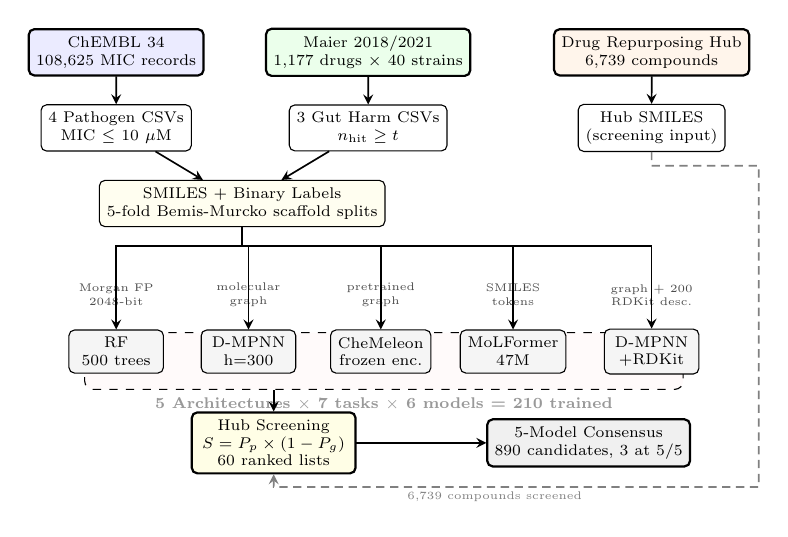
\begin{tikzpicture}[
  src/.style={rectangle, draw, rounded corners=2pt, minimum width=2.2cm,
              minimum height=0.55cm, font=\scriptsize, align=center, thick},
  proc/.style={rectangle, draw, rounded corners=2pt, minimum width=2.2cm,
               minimum height=0.55cm, font=\scriptsize, align=center},
  mdl/.style={rectangle, draw, rounded corners=2pt, minimum width=1.5cm,
              minimum height=0.45cm, font=\scriptsize, align=center, fill=black!4},
  outbox/.style={rectangle, draw, rounded corners=2pt, minimum width=2.6cm,
              minimum height=0.55cm, font=\scriptsize, align=center, thick},
  arr/.style={->, >=stealth, semithick},
  lbl/.style={font=\tiny, color=black!70, align=center},
  scale=0.80, transform shape
]
% Row 1: Data Sources
\node[src, fill=blue!8] (chembl) at (0, 6.5) {ChEMBL 34\\108,625 MIC records};
\node[src, fill=green!8] (maier) at (4, 6.5) {Maier 2018/2021\\1,177 drugs $\times$ 40 strains};
\node[src, fill=orange!8] (hub) at (8.5, 6.5) {Drug Repurposing Hub\\6,739 compounds};

% Row 2: Processing
\node[proc] (p1) at (0, 5.3) {4 Pathogen CSVs\\MIC $\leq$ 10 $\mu$M};
\node[proc] (p2) at (4, 5.3) {3 Gut Harm CSVs\\$n_{\mathrm{hit}} \geq t$};
\node[proc] (p3) at (8.5, 5.3) {Hub SMILES\\(screening input)};

\draw[arr] (chembl) -- (p1);
\draw[arr] (maier) -- (p2);
\draw[arr] (hub) -- (p3);

% Row 3: Common preparation
\node[proc, minimum width=4.2cm, fill=yellow!6] (common) at (2, 4.1)
  {SMILES + Binary Labels\\5-fold Bemis-Murcko scaffold splits};
\draw[arr] (p1) -- (common);
\draw[arr] (p2) -- (common);

% Row 4: Per-model featurization arrows into model group
\node[draw, dashed, rounded corners=3pt, inner sep=5pt,
      minimum width=9.5cm, minimum height=0.9cm,
      fill=red!2] (mgroup) at (4.25, 1.6) {};
\node[font=\scriptsize\bfseries, anchor=north, color=black!40]
  at (mgroup.south) {5 Architectures $\times$ 7 tasks $\times$ 6 models = 210 trained};

\node[mdl] (m1) at (0, 1.75) {RF\\500 trees};
\node[mdl] (m2) at (2.1, 1.75) {D-MPNN\\h=300};
\node[mdl] (m3) at (4.2, 1.75) {CheMeleon\\frozen enc.};
\node[mdl] (m4) at (6.3, 1.75) {MoLFormer\\47M};
\node[mdl] (m5) at (8.5, 1.75) {D-MPNN\\+RDKit};

% Featurization labels above each model, below the arrows
\node[lbl] at (0, 2.65) {Morgan FP\\2048-bit};
\node[lbl] at (2.1, 2.65) {molecular\\graph};
\node[lbl] at (4.2, 2.65) {pretrained\\graph};
\node[lbl] at (6.3, 2.65) {SMILES\\tokens};
\node[lbl] at (8.5, 2.65) {graph + 200\\RDKit desc.};

% Individual arrows from common to each model
\draw[arr] (common.south) -- ++(0,-0.3) -| (m1.north);
\draw[arr] (common.south) -- ++(0,-0.3) -| (m2.north);
\draw[arr] (common.south) -- ++(0,-0.3) -| (m3.north);
\draw[arr] (common.south) -- ++(0,-0.3) -| (m4.north);
\draw[arr] (common.south) -- ++(0,-0.3) -| (m5.north);

% Row 5: Outputs
\node[outbox, fill=yellow!10] (screen) at (2.5, 0.3)
  {Hub Screening\\$S = P_p \times (1 - P_g)$\\60 ranked lists};
\node[outbox, fill=black!6] (cons) at (7.5, 0.3)
  {5-Model Consensus\\890 candidates, 3 at 5/5};

\draw[arr] (mgroup.south -| screen.north) -- (screen.north);
\draw[arr] (screen) -- (cons);

% Hub -> Screening route (dashed, bypasses training)
\draw[arr, densely dashed, color=black!50]
  (p3.south) -- (8.5, 4.7) -- (10.2, 4.7) -- (10.2, -0.4) -- (2.5, -0.4) -- (screen.south);
\node[font=\tiny, color=black!50, anchor=west] at (4.5, -0.55) {6,739 compounds screened};
\end{tikzpicture}
\caption{Pipeline overview. Three data sources (top) are processed into SMILES-label pairs with shared 5-fold scaffold splits. Each model receives its own featurization of the same SMILES: Morgan fingerprints for RF, molecular graphs for D-MPNN and CheMeleon, SMILES tokens for MoLFormer, and graphs with 200 RDKit descriptors for D-MPNN+RDKit. All 210 trained models screen the Hub to produce 60 selectivity-ranked lists, aggregated into a multi-model consensus. The dashed path indicates that Hub compounds enter only at inference time.}
\label{fig:pipeline}
\end{figure*}

\subsection{Molecular Featurization and Cross-Validation}
\label{sec:features}

Morgan circular fingerprints (ECFP4; radius 2, 2,048 bits) are computed via RDKit for all compounds.
These serve as input features for the Random Forest model; the remaining four architectures learn their own molecular representations from SMILES or molecular graphs.

All models are evaluated using identical 5-fold Bemis-Murcko scaffold splits.
The Bemis-Murcko scaffold extracts the core ring system and linkers, stripping side chains; all compounds sharing a scaffold are assigned to the same fold, ensuring that the test set contains structurally novel compounds not seen during training.

For each task, five fold-specific models are trained for cross-validation evaluation, plus one final model trained on 100\% of the data for Hub screening.
Total: $7 \text{ tasks} \times 6 \text{ models} \times 5 \text{ architectures} = 210$ trained models.

\subsection{Model Architectures}
\label{sec:models}

\paragraph{Baseline and motivation.}
The primary baseline is the Stokes et al.~\citep{stokes2020} pipeline: a single D-MPNN~\citep{yang2019} augmented with 200 RDKit 2D molecular descriptors, trained on 2,335 compounds for a single pathogen (\textit{E.~coli}), optimized for pathogen-killing probability alone, and evaluated with random train/test splits.
Key features of that baseline include the Chemprop D-MPNN graph neural network architecture, Morgan fingerprint and RDKit descriptor molecular representations, and binary growth-inhibition labels from phenotypic screening.
The motivation is directly from the Stokes et al.\ discussion, which noted that training across phylogenetically diverse species may make it possible to predict molecules with activity against a specified spectrum of pathogens, raising the prospect of narrow-spectrum agents that can be administered systemically without damaging the host microbiota~\citep{stokes2020}.
We attempt to take a step toward that vision by extending the baseline in four directions:
(i)~\emph{dual-objective scoring}: we add a gut commensal harm model trained on the Maier et al.~\citep{maier2018} screen of 1,177 drugs against 40 gut strains, combining pathogen and gut predictions into a selectivity score $S = P_p \times (1 - P_g)$ that the baseline does not include;
(ii)~\emph{multi-pathogen coverage}: we scale from 1 pathogen to 4 WHO-priority pathogens (108,625 training instances, 8--19$\times$ larger per pathogen);
(iii)~\emph{architectural diversity}: we train 5 architecturally different models (RF, D-MPNN, CheMeleon, MoLFormer-XL, D-MPNN+RDKit), each capturing different molecular representations; and
(iv)~\emph{multi-model consensus}: we aggregate predictions across all five architectures to identify candidates that are robust to any single model's biases.

Five architecturally diverse models are trained independently on identical data and splits.
Architectural details and hyperparameters are summarized in Table~\ref{tab:architectures}; extended descriptions appear in Supplementary Material~\ref{app:models}.

\begin{table}[t]
\caption{Summary of five model architectures. Parameters listed are per model; model size is the saved checkpoint.}
\label{tab:architectures}
\vskip 0.1in
\centering
\scriptsize
\begin{tabular}{llrr}
\toprule
\textbf{Model} & \textbf{Input representation} & \textbf{Params} & \textbf{Size} \\
\midrule
RF + Morgan FP & 2,048-bit ECFP4 & 500 trees & 6--383 MB \\
D-MPNN & Molecular graph & ${\sim}$200K & 1.6 MB \\
CheMeleon (frozen) & Molecular graph & ${\sim}$615K\textsuperscript{a} & 37.4 MB \\
MoLFormer-XL & SMILES string & ${\sim}$47M & 177.7 MB \\
D-MPNN+RDKit & Graph + 200 desc. & ${\sim}$3.4M & 43.3 MB \\
\bottomrule
\end{tabular}
\vskip 0.05in
\raggedright\scriptsize\textsuperscript{a}Trainable parameters only; total including frozen encoder is ${\sim}$9.3M (8.7M encoder + ${\sim}$615K classification head).
\end{table}

\paragraph{Random Forest (RF).}
An ensemble of 500 decision trees trained on 2,048-bit Morgan fingerprints with balanced class weighting.
Feature subsampling (square root of total features per split) and a minimum leaf size of 2 provide regularization.
Probability estimates are computed as the fraction of trees voting active, yielding well-calibrated scores that serve as the strongest individual-model baseline.

\paragraph{D-MPNN.}
A directed message-passing neural network~\citep{yang2019} implemented in Chemprop v2.2.2~\citep{chemprop2024} with depth 3, hidden size 300, and dropout 0.1.
The model learns molecular representations by iteratively passing messages along directed bonds, aggregating atom-level information into a molecule-level vector that is passed through a feed-forward network (FFN) for classification.
Approximately 200K parameters per model.

\paragraph{CheMeleon (frozen encoder).}
CheMeleon~\citep{chemeleon2024} is a recent molecular foundation model (Burns et al., 2025) that pretrains a D-MPNN backbone (6 message-passing layers, hidden dimension 2,048, 8.7M parameters) on 1,613 deterministic Mordred descriptors computed from PubChem compounds.
It adds a pretrained graph representation to the pipeline, complementing RF (fixed fingerprints), vanilla D-MPNN (graph learned from scratch), MoLFormer (pretrained SMILES transformer), and D-MPNN+RDKit (graph plus descriptors).
Full fine-tuning of the 9.3M-parameter model on our smallest dataset (1,177 Maier gut compounds) would yield a parameter-to-sample ratio exceeding 7,900:1; preliminary experiments confirmed that a learning rate of $10^{-3}$ destroyed pretrained weights within 2--3 epochs.
We therefore freeze the encoder weights entirely and train only a binary classification head (${\sim}$615K parameters), following the standard transfer learning paradigm.
This approach is approximately 10$\times$ faster than full fine-tuning and eliminates encoder overfitting on small datasets.

\paragraph{MoLFormer-XL.}
A BERT-style transformer~\citep{molformer2022} pretrained on 1.1 billion SMILES strings from ZINC and PubChem using masked language modeling.
The model tokenizes SMILES strings and produces contextual embeddings that are fine-tuned for each classification task.
At approximately 47M parameters, it is the largest model in the pipeline.

\paragraph{D-MPNN+RDKit.}
This model follows the architecture of Stokes et al.~\citep{stokes2020}: a D-MPNN augmented with 200 RDKit 2D molecular descriptors (MW, LogP, TPSA, HBD, HBA, rotatable bonds, ring counts, and other physicochemical properties), configured with depth 5, hidden size 1,600, and dropout 0.35.
The RDKit descriptors are concatenated with the graph-learned molecular vector before the FFN, providing explicit physicochemical context.
At approximately 3.4M parameters (43.3 MB per model), it is 17$\times$ larger than the vanilla D-MPNN.
This model was added to address two calibration patterns observed in the vanilla D-MPNN: probability saturation (61.6\% of Hub compounds receiving $S < 0.01$) and phosphate enrichment (3.05$\times$ overweighting of phosphate-containing compounds in the top-50).

\paragraph{Computing infrastructure.}
All training and inference were performed on the Ada HPC cluster at IIIT Hyderabad (partition u22) using NVIDIA GeForce RTX 2080 Ti GPUs (11 GB), managed via SLURM.
RF training used CPU only (scikit-learn).
D-MPNN, CheMeleon (frozen encoder), and MoLFormer-XL each trained on a single RTX 2080 Ti; D-MPNN+RDKit used 3 GPUs in parallel (2$\times$ RTX 2080 Ti, 1$\times$ RTX 4070) via a GPU pool.
All neural models used PyTorch 2.4.1 with CUDA 11.8.

\subsection{Selectivity Score}
\label{sec:selectivity}

For each Hub compound, each trained model independently predicts the probability of pathogen activity ($\pp$) and the probability of gut harm ($\pg$).
These are combined into a selectivity score:
\begin{equation}
S = \pp \times (1 - \pg)
\label{eq:selectivity}
\end{equation}
A compound receives high $S$ only if it is simultaneously predicted to kill the target pathogen ($\pp \to 1$) and spare gut commensals ($\pg \to 0$).
Neither axis alone suffices: a potent but gut-toxic compound receives low $S$ due to the $(1 - \pg)$ penalty, while a gut-safe but inactive compound receives low $S$ due to low $\pp$.

With 5 models, 4 pathogens, and 3 gut thresholds, the pipeline produces $5 \times 4 \times 3 = 60$ selectivity-ranked lists, plus 21 raw prediction CSVs, totaling 81 screening output files.

Threshold sensitivity is assessed by computing Spearman rank correlations between selectivity rankings at different $t$ values.
If $\rho(S_{t{=}5}, S_{t{=}20}) > 0.9$ for a given model and pathogen, the selectivity ranking is considered robust to the specific definition of gut harm.

\subsection{Multi-Model Consensus}
\label{sec:consensus}

The consensus framework exploits architectural diversity to identify compounds that are robust to model-specific biases.
For each of the 60 ranked lists, the top-50 compounds by $S$ are selected.
A compound's consensus tier is the number of models (out of 5) that independently place it in their respective top-50 for any pathogen-threshold combination.

\paragraph{Rationale.}
Each model exhibits characteristic calibration patterns: D-MPNN shows probability saturation and phosphate enrichment, CheMeleon favors low-MW molecules, MoLFormer exhibits heavy saturation (53\% near-zero $S$), and D-MPNN+RDKit shows residual phosphate preference for MTB.
Pairwise top-100 Jaccard overlap ranges from 0.02 to 0.16 across model pairs, confirming that the five architectures capture largely independent aspects of molecular structure.
A compound reaching tier 5/5 has been independently identified by models using fundamentally different molecular representations (fixed fingerprints, learned graphs, pretrained graph embeddings, sequential SMILES patterns, and graph-plus-descriptor hybrids), making it unlikely that any single model's bias produced the agreement.

\paragraph{Disagreement metric.}
For each compound appearing in any model's top-50, we compute the selectivity percentile (rank / 6,739) for each of the five models and report the standard deviation of these percentiles as the \emph{disagreement} score.
Low disagreement indicates that all models assign similar relative rankings, providing a continuous measure of consensus confidence beyond the discrete tier count.

% ============================================================
% PLACEHOLDER FOR REMAINING SECTIONS
% ============================================================

% ============================================================
% 4. RESULTS
% ============================================================

\section{Results}
\label{sec:results}

\subsection{Cross-Validation Performance}
\label{sec:cv}

Table~\ref{tab:rocauc} reports 5-fold scaffold cross-validation ROC-AUC for all five models across seven tasks.
Extended metrics (PR-AUC, MCC, sensitivity, specificity) are provided in Supplementary Material~\ref{app:extended_metrics}.

\begin{table}[t]
\caption{ROC-AUC (mean $\pm$ std) across 5-fold Bemis-Murcko scaffold CV. Best per task in \textbf{bold}. Green cells indicate task winner.}
\label{tab:rocauc}
\vskip 0.1in
\centering
\scriptsize
\setlength{\tabcolsep}{3pt}
\begin{tabular}{lccccc}
\toprule
\textbf{Task} & \textbf{RF} & \textbf{D-MPNN} & \textbf{CheMel} & \textbf{MoLF} & \textbf{+RDKit} \\
\midrule
\textit{E.~coli}      & \textbf{.877}{\tiny$\pm$.011} & .853{\tiny$\pm$.012} & .833{\tiny$\pm$.011} & .838{\tiny$\pm$.018} & .841{\tiny$\pm$.014} \\
\textit{S.~aureus}    & \textbf{.871}{\tiny$\pm$.007} & .854{\tiny$\pm$.013} & .831{\tiny$\pm$.010} & .835{\tiny$\pm$.015} & .839{\tiny$\pm$.009} \\
\textit{P.~aerug.}    & \textbf{.861}{\tiny$\pm$.014} & .838{\tiny$\pm$.013} & .820{\tiny$\pm$.018} & .828{\tiny$\pm$.011} & .823{\tiny$\pm$.014} \\
\textit{M.~tb}        & \textbf{.811}{\tiny$\pm$.018} & .760{\tiny$\pm$.023} & .762{\tiny$\pm$.013} & .764{\tiny$\pm$.018} & .738{\tiny$\pm$.031} \\
\midrule
Gut ($t{=}5$)  & .804{\tiny$\pm$.073} & .825{\tiny$\pm$.051} & .826{\tiny$\pm$.039} & .847{\tiny$\pm$.041} & \textbf{.849}{\tiny$\pm$.054} \\
Gut ($t{=}10$) & .823{\tiny$\pm$.090} & \textbf{.841}{\tiny$\pm$.039} & .812{\tiny$\pm$.071} & .822{\tiny$\pm$.064} & .829{\tiny$\pm$.091} \\
Gut ($t{=}20$) & \textbf{.880}{\tiny$\pm$.050} & .878{\tiny$\pm$.072} & .858{\tiny$\pm$.076} & .862{\tiny$\pm$.067} & .856{\tiny$\pm$.112} \\
\bottomrule
\end{tabular}
\end{table}

RF achieves the highest ROC-AUC on all four pathogen tasks (0.811--0.877) and gut $t{=}20$ (0.880), serving as the natural baseline: the simplest architecture (fixed fingerprints, no learned representations) against which the four neural models are compared.
No single model dominates the gut tasks: D-MPNN+RDKit wins $t{=}5$ (0.849), D-MPNN wins $t{=}10$ (0.841), and RF wins $t{=}20$ (0.880).
\textit{M.~tuberculosis} is the hardest task across all models (0.738--0.811), consistent with MTB's chemically distinct training data (lower MW, higher LogP than Gram-negative pathogens).
Gut task variance is substantially higher ($\pm$0.05--0.11 vs $\pm$0.01--0.03 for pathogens), reflecting the small Maier dataset (1,177 compounds, approximately 235 per fold).

The complementarity of model strengths motivates the multi-model consensus: RF excels where training data is abundant (18K--44K pathogen compounds), while neural models are competitive on the smaller Maier dataset.

\subsection{Screening and Calibration Analysis}
\label{sec:screening}

Virtual screening of the 6,739 Hub compounds reveals substantial differences in model calibration (Table~\ref{tab:calibration}).
RF distributes selectivity scores across the full $[0,1]$ range, with only 14 compounds (0.2\%) receiving near-zero $S$ ($< 0.01$).
In contrast, the vanilla D-MPNN assigns 4,153 compounds (61.6\%) to $S < 0.01$, concentrating the selectivity ranking in a narrow subset of the screening library.
This saturation arises because the D-MPNN's learned graph representations collapse to extreme values for compounds structurally distant from the training data.

\begin{table}[t]
\caption{Selectivity score distribution for \textit{E.~coli} ($t{=}10$) across 6,739 Hub compounds.}
\label{tab:calibration}
\vskip 0.1in
\centering
\scriptsize
\begin{tabular}{lrrr}
\toprule
\textbf{Model} & $S{<}0.01$ & \textbf{Mid-range} & $S{>}0.95$ \\
\midrule
RF              & \textbf{14} (0.2\%) & \textbf{1,941} & 0 \\
D-MPNN          & 4,153 (61.6\%) & 646 & 114 \\
CheMeleon       & 742 (11.0\%) & 1,440 & 9 \\
MoLFormer       & 3,571 (53.0\%) & 826 & 36 \\
D-MPNN+RDKit    & 212 (3.1\%) & 1,612 & 0 \\
\bottomrule
\end{tabular}
\end{table}

The D-MPNN+RDKit model addresses both calibration patterns: near-zero predictions drop from 4,153 to 212 (95\% reduction), and phosphate-containing compounds in the top-50 drop from 40\% to 4\% (Hub baseline: 2.3\%).
The 200 RDKit descriptors provide a physicochemical anchor that regularizes predictions for compounds structurally distant from training data, while diluting the graph's overconfidence in the phosphate substructure pattern.
Top-50 overlap between the old D-MPNN and D-MPNN+RDKit is only 1 compound, indicating a fundamentally different ranking.

Threshold sensitivity analysis confirms that selectivity rankings are robust across gut thresholds: Spearman $\rho$ between $S_{t{=}5}$ and $S_{t{=}20}$ exceeds 0.91 for all model-pathogen combinations, with a minimum of 0.859 (D-MPNN+RDKit, MTB).

\subsection{External Validation}
\label{sec:external}

We validate against 4,343 compounds for which Stokes et al.~\citep{stokes2020} published D-MPNN prediction scores (Table S2 of the original paper).
For each of our five models, we compute Spearman $\rho$ between our predicted $\pp$ and the Stokes D-MPNN score, and separately between our selectivity $S$ and the same Stokes score (Table~\ref{tab:stokes}).

\begin{table}[t]
\caption{Spearman $\rho$ vs Stokes D-MPNN scores ($n{=}4{,}343$). Gap = $\rho(\pp) - \rho(S)$ measures the gut penalty effect.}
\label{tab:stokes}
\vskip 0.1in
\centering
\scriptsize
\begin{tabular}{lccc}
\toprule
\textbf{Model} & $\rho(\pp)$ & $\rho(S)$ & \textbf{Gap} \\
\midrule
RF              & \textbf{0.363} & 0.177 & \textbf{0.186} \\
D-MPNN+RDKit    & 0.331 & 0.187 & 0.145 \\
MoLFormer       & 0.261 & 0.189 & 0.072 \\
CheMeleon       & 0.260 & 0.161 & 0.099 \\
D-MPNN          & 0.235 & 0.154 & 0.081 \\
\bottomrule
\end{tabular}
\end{table}

All $\rho(\pp)$ values are positive and highly significant, confirming that our pathogen activity predictions align with independently obtained laboratory measurements.
RF achieves the highest correlation ($\rho = 0.363$), and D-MPNN+RDKit shows a 41\% improvement over vanilla D-MPNN (0.331 vs 0.235), validating the architectural enhancement.

The gap $\rho(\pp) - \rho(S)$ quantifies the effectiveness of the gut penalty.
RF shows the largest gap (0.186): compounds that Stokes ranks highly but that also harm gut bacteria are penalized most strongly by the $(1 - \pg)$ term.
This is consistent with the selectivity framework operating as designed, preferentially down-weighting broad-spectrum compounds.

A separate validation against 616 compounds with Stokes RF scores yields RF-to-RF $\rho(\pp) = 0.500$, the strongest external validation signal in the pipeline.

\paragraph{Halicin case study.}
Halicin (SU3327), the flagship discovery of Stokes et al., is a broad-spectrum antibiotic that kills \textit{E.~coli}, \textit{M.~tuberculosis}, \textit{A.~baumannii}, and \textit{C.~difficile} by disrupting the transmembrane proton gradient.
Our pipeline assigns $S < 0.13$ across all five models (RF: 0.085, D-MPNN: 0.000, CheMeleon: 0.000, MoLFormer: 0.007, D-MPNN+RDKit: 0.125), consistently placing halicin outside the top selective candidates.
The RF decomposition reveals moderate pathogen activity ($\pp = 0.173$) coupled with high gut harm ($\pg = 0.509$), yielding $S = 0.173 \times (1 - 0.509) = 0.085$.
Inter-model disagreement is 0.236 (moderate): models differ on the degree of penalization but unanimously agree that halicin is not a top-tier selective candidate.
This is consistent with the pipeline not simply rediscovering broad-spectrum antibiotics.

\subsection{Multi-Model Consensus}
\label{sec:consensus_results}

Of 6,739 Hub compounds, 890 unique compounds appear in at least one model's top-50 across all pathogen-threshold combinations.
The consensus tier distribution is: 3 at 5/5, 9 at 4/5, 40 at 3/5, 183 at 2/5, and 655 at 1/5.
Of these, 58 (6.5\%) are classified as known antibiotics in the Hub; the remaining 832 (93.5\%) are novel.

Table~\ref{tab:consensus} presents the 12 compounds reaching tier 4 or above.
Eight of 12 possess antibiotic-relevant mechanisms of action (protein synthesis inhibition, cell wall synthesis, topoisomerase inhibition, LeuRS inhibition, DprE1 inhibition).
Three are aminoglycosides (micronomicin, netilmicin, sisomicin) with clinically established narrow-spectrum profiles, providing biological validation of the selectivity framework.
SQ-109 and macozinone are in clinical development for tuberculosis; gepotidacin (topoisomerase inhibitor) is in Phase~2 for urinary tract infections.

\begin{table}[t]
\caption{Consensus tier 4+/5 candidates. Phase: clinical development stage. Pathogens: number of pathogen tasks where the compound appears in top-50. Best $S$: maximum selectivity score across all model-pathogen-threshold combinations.}
\label{tab:consensus}
\vskip 0.1in
\centering
\scriptsize
\setlength{\tabcolsep}{2.5pt}
\begin{tabular}{llccl}
\toprule
\textbf{Compound} & \textbf{Phase} & \textbf{Path.} & \textbf{Best $S$} & \textbf{MoA} \\
\midrule
\multicolumn{5}{l}{\textit{Tier 5/5 (all models agree):}} \\
retapamulin   & Launched & 2 & 0.9995 & Protein synth. (pleuromutilin) \\
AFN-1252      & Phase 2  & 2 & 0.9979 & FabI inhibitor \\
trimetrexate  & Phase 3  & 3 & 0.9924 & DHFR inhibitor \\
\midrule
\multicolumn{5}{l}{\textit{Tier 4/5 (9 compounds):}} \\
micronomicin  & Launched & 4 & 0.9998 & Aminoglycoside \\
SQ-109        & Phase 3  & 1 & 0.9998 & Cell wall synth. \\
netilmicin    & Launched & 4 & 0.9995 & Aminoglycoside \\
macozinone    & Preclin. & 1 & 0.9994 & DprE1 inhibitor \\
GSK656        & Preclin. & 3 & 0.9954 & LeuRS inhibitor \\
gepotidacin   & Phase 2  & 3 & 0.9935 & Topoisomerase inh. \\
vinburnine    & Launched & 1 & 0.9930 & Adrenergic rec. ant. \\
sisomicin     & Launched & 4 & 0.9886 & Aminoglycoside \\
SB-772077B    & Preclin. & 2 & 0.9749 & ROCK inhibitor \\
\bottomrule
\end{tabular}
\end{table}

Eight compounds are independently placed above the 95th selectivity percentile by all five models.
AFN-1252 (FabI inhibitor, Phase~2) achieves the lowest disagreement score (0.008), with all five models placing it in the top 0.1--2.3\% of Hub compounds.

% ============================================================
% 5. DISCUSSION
% ============================================================

\section{Discussion}
\label{sec:discussion}

\paragraph{RF dominance on pathogen tasks.}
The simplest model (RF with fixed Morgan fingerprints) consistently outperforms four neural architectures on pathogen tasks.
This likely reflects the large training sets (18K--44K compounds) with active fractions of 26--44\%, substantially higher than the approximately 5\% in Stokes et al.~\citep{stokes2020}.
At this scale and class balance, the 2,048-bit fingerprint provides sufficient molecular resolution and the 500-tree ensemble produces well-calibrated probabilities.
Neural models may offer advantages on smaller or more structurally diverse datasets, as evidenced by their competitive performance on the 1,177-compound Maier gut tasks.

\paragraph{Calibration and discrimination.}
The D-MPNN+RDKit model illustrates a key distinction: while its ROC-AUC (discrimination) is comparable to the vanilla D-MPNN, it substantially improves calibration (the meaningfulness of absolute probability values).
For selectivity screening, calibration is particularly important because the $S$ score is a product of two probabilities.
Models with concentrated score distributions (e.g., 61.6\% near-zero for D-MPNN) yield $S$ values that do not differentiate the majority of compounds, whereas well-calibrated models distribute scores across the full $[0,1]$ range.

\paragraph{Biological validation.}
The enrichment of aminoglycosides (micronomicin, netilmicin, sisomicin) in the top consensus tiers provides biological validation.
Aminoglycosides are clinically known to be narrow-spectrum: they target the 30S ribosomal subunit and are taken up by specific bacterial transport mechanisms that most gut commensals lack.
Their presence at tier 4/5 is consistent with the selectivity framework surfacing compounds with microbiome-sparing properties.

The halicin case study provides complementary negative validation: a known broad-spectrum antibiotic receives low $S$ across all models, demonstrating that the pipeline does not trivially rediscover potent-but-destructive compounds.

\paragraph{Known drug validation.}
As a sanity check, we verify that known narrow-spectrum drugs (daptomycin, fidaxomicin, methenamine, nitrofurantoin) receive higher mean $S$ than known broad-spectrum drugs (amoxicillin, ciprofloxacin, chloramphenicol, clindamycin, doxycycline, rifabutin).
RF confirms the expected direction (narrow mean $S = 0.163$ vs broad $S = 0.087$), reinforcing its role as the most reliable individual model.

\paragraph{Scope and methodological considerations.}
All results are computational predictions; the candidates identified here are positioned for experimental follow-up.
The gut harm model is trained on monoculture screening data from Maier et al.; Garc\'{i}a-Santamarina et al.~\citep{garcia2024} demonstrated that cross-protection is the dominant emergent community behavior (6$\times$ more frequent than cross-sensitization), indicating that monoculture-based predictions represent a conservative upper bound on actual gut harm.
The selectivity composition $S = \pp \times (1 - \pg)$ operates on model predictions derived from molecular structure; both the pathogen and gut models take the same SMILES input and produce probabilities, so compound-level overlap between training sets is seldom required for the composition to produce meaningful rankings.
Our Fisher exact test analysis supports the dual-objective approach: pathogen activity and gut harm are significantly associated for Gram-negative and Gram-positive pathogens (OR 7.7--13.1, $p < 0.01$), suggesting that the $(1 - \pg)$ penalty addresses a real biological correlation.
For \textit{M.~tuberculosis}, the absence of significant association (OR 1.9, $p = 0.37$) indicates that selectivity is biologically achievable, and the framework reflects this asymmetry.
Screening is restricted to the Drug Repurposing Hub (6,739 compounds with established safety profiles and synthesis routes), which facilitates experimental follow-up but does not cover structurally novel scaffolds outside pharmaceutical chemical space.

\paragraph{Comparison with prior computational approaches.}
Zheng et al.~\citep{zheng2019}, McCoubrey et al.~\citep{mccoubrey2021}, and Algavi \& Borenstein~\citep{algavi2023} built gut harm prediction models achieving AUROC 0.81--0.86, but did not integrate pathogen activity prediction.
Our gut task ROC-AUC (0.80--0.88 across models and thresholds) is comparable, while our framework additionally provides the $\pp$ predictions, the combined selectivity score, and multi-model consensus.
The primary contribution of this work is the dual-objective integration and multi-architecture consensus that together produce high-confidence selective candidates.

\paragraph{Research Outlook.}
The monoculture-based gut model could be extended with community-level interaction data as it becomes available, building on the cross-protection findings of Garcia-Santamarina et al.~\citep{garcia2024}.
Dose-response modeling, replacing the binary MIC threshold with continuous potency estimates, would refine the selectivity score for compounds near the decision boundary.
Expanding the screening library beyond the Drug Repurposing Hub to larger virtual libraries (e.g., ZINC15, Enamine REAL) would access structurally novel scaffolds outside established pharmaceutical chemical space.
% ============================================================
% 6. CONCLUSION
% ============================================================

\section{Conclusion}
\label{sec:conclusion}

We have presented a multi-architecture consensus pipeline for microbiome-sparing antibiotic discovery that jointly predicts pathogen-killing efficacy and gut commensal harm from molecular structure.
Five architecturally diverse models, trained on 108,625 pathogen activity instances and 1,177 gut harm compounds across seven binary classification tasks, produce 60 selectivity-ranked screening lists for 6,739 Drug Repurposing Hub compounds.

The pipeline identifies 3 compounds with unanimous 5/5 model agreement and 8 compounds above the 95th selectivity percentile in all five models, with inter-model disagreement as low as 0.008.
External validation against 4,343 Stokes et al.\ lab-scored compounds confirms alignment of pathogen predictions ($\rho = 0.363$) and effective gut penalty operation.
The halicin case study demonstrates correct penalization of a known broad-spectrum antibiotic ($S < 0.13$ across all models).

By treating selectivity as an explicit optimization target, the framework offers a computational complement to the experimental discoveries of lolamicin~\citep{munoz2024} and enterololin~\citep{catacutan2025}, which achieved microbiome-sparing selectivity through large-scale screening campaigns.

% ============================================================
% 7. CODE, DATA, AND VISUALIZATIONS
% ============================================================

\section{Code, Data, and Visualizations}
\label{sec:resources}

All pipeline code, training data, screening results, and analysis outputs are publicly available at:

\begin{center}
\small
\url{https://github.com/VishakhaAgrawal27/2023101040_MLNS_CourseProject}
\end{center}

\noindent The 66 interactive HTML visualizations (3D selectivity surfaces, candidate landscapes, consensus heatmaps, ranked list explorers, and model diagnostics) are deployed at:

\begin{center}
\small
\url{https://web.iiit.ac.in/~vishakha.agrawal/viz/other/mlns/}
\end{center}

% ============================================================
% ACKNOWLEDGEMENTS
% ============================================================

\section*{Acknowledgements}

This work was carried out in partial fulfillment of the requirements of the course project for Machine Learning for Natural Sciences, Spring 2026, at the International Institute of Information Technology, Hyderabad.
We thank Dr.\ Vinod P.\ K.\ and Dr.\ Prabhakar Bhimalapuram for their instruction and guidance throughout the duration of the course.
All experiments were performed on the Ada HPC cluster at IIIT Hyderabad.

% ============================================================
% REFERENCES
% ============================================================
\bibliography{references_v2}
\bibliographystyle{icml2025}


% ============================================================
% APPENDIX
% ============================================================
\newpage
\appendix
\renewcommand{\appendixname}{Supplementary Material}

\section{Dataset Details}
\label{app:data}

\subsection{Pathogen Dataset Statistics}

\begin{table}[ht]
\caption{Pathogen dataset statistics from ChEMBL 34. N: total compounds after deduplication. Active: compounds with median MIC $\leq$ 10 $\mu$M. Median molecular properties (MW in Da, LogP, TPSA in \AA$^2$) characterize each dataset's chemical space.}
\label{tab:pathogen_detail}
\centering
\scriptsize
\setlength{\tabcolsep}{3pt}
\begin{tabular}{lrrrrr}
\toprule
\textbf{Pathogen} & \textbf{N} & \textbf{Active} & \textbf{\%} & \textbf{Med. MW} & \textbf{vs Stokes} \\
\midrule
\textit{E.~coli}         & 28,284 & 9,249  & 32.7 & 437 Da & 12.1$\times$ \\
\textit{S.~aureus}       & 43,853 & 19,267 & 43.9 & 443 Da & 18.8$\times$ \\
\textit{P.~aeruginosa}   & 17,783 & 4,657  & 26.2 & 446 Da & 7.6$\times$ \\
\textit{M.~tuberculosis} & 18,705 & 8,129  & 43.5 & 391 Da & 8.0$\times$ \\
\midrule
\textbf{Total instances}  & \textbf{108,625} & \textbf{41,302} & 38.0 & & \\
\textbf{Unique compounds} & \textbf{67,155} & & & & \\
\bottomrule
\end{tabular}
\end{table}

MIC measurements were obtained from ChEMBL~\citep{chembl34} via its REST API, retaining records with standard type ``MIC,'' valid units (nM or $\mu$g/mL), and relations $=$, $\leq$, or $<$.
For compounds with replicate measurements, the median MIC was taken.
Activity threshold: MIC $\leq$ 10,000 nM (10 $\mu$M), a standard threshold consistent with prior antibiotic discovery work~\citep{stokes2020,wong2024}.

The 108,625 total includes compounds that appear in multiple pathogen datasets due to multi-organism assays (e.g., a compound tested against both \textit{E.~coli} and \textit{S.~aureus} counts once per dataset; 67,155 unique SMILES remain after deduplication).
\textit{M.~tuberculosis} is chemically distinct from the other three: lower median MW (391 vs 437--446 Da), higher mean LogP (3.85 vs 3.0--3.5), and lower mean TPSA, reflecting the smaller, more lipophilic molecules required to penetrate the mycobacterial cell wall.

\begin{figure}[ht]
\centering

\includegraphics[width=\columnwidth]{figures/data_class_balance.png}
\caption{Class balance across all seven binary classification tasks. Pathogen active fractions range from 26.2\% (\textit{P.~aeruginosa}) to 43.9\% (\textit{S.~aureus}). Gut harm prevalence decreases with threshold stringency: 19.8\% ($t{=}5$), 15.2\% ($t{=}10$), 10.8\% ($t{=}20$).}
\label{fig:class_balance}
\end{figure}

\subsection{Gut Commensal Harm Data}

The gut harm labels derive from the systematic drug-microbiome screens of Maier et al.~\citep{maier2018,maier2021}.
The 2018 study screened 1,197 marketed drugs from the Prestwick Chemical Library against 40 representative gut bacterial strains in anaerobic monoculture at estimated intestinal concentrations.
The 2021 study extended this with quantitative MIC characterization of 144 antibiotics across 27 strains, establishing inter-source data compatibility.
Both datasets' supplementary files were used in our pipeline.
After SMILES canonicalization and deduplication, 1,177 compounds with valid structures were retained.

\begin{table}[ht]
\caption{Taxonomic distribution of 40 gut bacterial strains from the Maier et al.\ screen. Firmicutes (19 strains) and Bacteroidetes (12 strains) dominate, reflecting the major phyla of the healthy human gut. Gram-positive and Gram-negative strains are approximately balanced (23 vs 17).}
\label{tab:gut_strains}
\centering
\scriptsize
\begin{tabular}{lrl}
\toprule
\textbf{Phylum} & \textbf{Strains} & \textbf{Gram stain} \\
\midrule
Firmicutes & 19 & Positive \\
Bacteroidetes & 12 & Negative \\
Actinobacteria & 4 & Positive \\
Proteobacteria & 3 & Negative \\
Verrucomicrobia & 1 & Negative \\
Fusobacteria & 1 & Negative \\
\midrule
\textbf{Total} & \textbf{40} & 23 G+, 17 G$-$ \\
\bottomrule
\end{tabular}
\end{table}

Strain sensitivity varies widely: \textit{Eubacterium rectale} is the most sensitive (inhibited by 236 drugs), while \textit{Bilophila wadsworthia} is the most resistant (81 drugs).
\textit{C.~difficile} (strain NT5083) ranks 23rd with 152 drugs causing inhibition.

\begin{figure}[ht]
\centering

\includegraphics[width=\columnwidth]{figures/data_maier_strain_sensitivity.png}
\caption{Per-strain sensitivity: number of drugs inhibiting each of the 40 gut strains. \textit{E.~rectale} is most sensitive (236 drugs); \textit{B.~wadsworthia} is most resistant (81 drugs).}
\label{fig:strain_sensitivity}
\end{figure}

The $n_{\mathrm{hit}}$ distribution is heavily right-skewed: 780 compounds (66.3\%) harm zero strains, 88 (7.5\%) harm exactly one, and 11 compounds inhibit all 40.
The 11 pan-active compounds are: rifabutin, doxycycline, chlortetracycline, tosufloxacin, chloramphenicol, minocycline, meclocycline, demeclocycline, methacycline (all antibiotics), chlorhexidine (antiseptic), and florfenicol (veterinary anti-infective).

Drug class analysis: antiseptics have the highest mean $n_{\mathrm{hit}}$ (28.2, 91.7\% harming at least one strain), followed by veterinary anti-infectives (22.2, 75.0\%), antibiotics (21.5, 77.5\%), antiprotozoals (10.6, 65.0\%), antifungals (9.0, 56.0\%), antiparasitics (6.6, 56.0\%), antivirals (2.2, 41.0\%), human-targeted drugs (1.4, 24.7\%), and non-drugs (0.7, 12.6\%).
The finding that 24.7\% of human-targeted (non-antibiotic) drugs inhibit at least one gut strain motivates training on the full 1,177 compounds rather than antibiotics alone.

\begin{table}[ht]
\caption{Binary gut harm labels at three thresholds ($t = 5, 10, 20$ strains inhibited). Higher thresholds capture progressively stricter definitions of microbiome disruption, reducing the harmful class from 19.8\% to 10.8\%.}
\label{tab:gut_thresholds}
\centering
\scriptsize
\begin{tabular}{cccl}
\toprule
$t$ & \textbf{Harmful} & \textbf{Harmful \%} & \textbf{Interpretation} \\
\midrule
5  & 233 & 19.8\% & Any substantial disruption \\
10 & 179 & 15.2\% & Quarter of tested strains affected \\
20 & 127 & 10.8\% & Broad devastation (half or more) \\
\bottomrule
\end{tabular}
\end{table}

\begin{figure}[ht]
\centering

\includegraphics[width=\columnwidth]{figures/data_maier_nhit.png}
\caption{Distribution of $n_{\mathrm{hit}}$ (number of gut strains inhibited) across 1,177 Maier compounds. The three dashed lines indicate the binary classification thresholds at $t = 5, 10, 20$.}
\label{fig:nhit}
\end{figure}

\subsection{Drug Repurposing Hub}

The Drug Repurposing Hub~\citep{repurposinghub} provides 6,739 compounds: Launched (2,393), Preclinical (2,297), Phase~2 (810), Phase~1 (565), Phase~3 (450), Withdrawn (95), with smaller transitional categories.
The Hub encompasses 1,432 unique mechanisms of action across 214 disease areas; the most represented are infectious disease (420), neurology/psychiatry (339), cardiology (202), endocrinology (121), and gastroenterology (119).

\subsection{Cross-Dataset Overlap}

\begin{table}[ht]
\caption{Pairwise compound overlap across all datasets (canonical SMILES match). Gram-negative and Gram-positive pathogen datasets share 79--87\% of compounds, while \textit{M.~tuberculosis} shares only 7--12\%, reflecting its distinct chemical space. The Hub-Maier overlap (478 compounds) provides a natural bridge for selectivity evaluation.}
\label{tab:overlap}
\centering
\scriptsize
\resizebox{\columnwidth}{!}{\begin{tabular}{lrrrrrr}
\toprule
& \textbf{Ec} & \textbf{Sa} & \textbf{Pa} & \textbf{Mtb} & \textbf{Maier} & \textbf{Hub} \\
\midrule
\textbf{Ec}    & 28,284 & 22,400 & 15,415 & 1,749 & 46  & 249 \\
\textbf{Sa}    &        & 43,853 & 14,928 & 2,304 & 59  & 314 \\
\textbf{Pa}    &        &        & 17,783 & 1,231 & 36  & 152 \\
\textbf{Mtb}   &        &        &        & 18,705& 57  & 147 \\
\textbf{Maier} &        &        &        &       & 1,177& 478 \\
\textbf{Hub}   &        &        &        &       &     & 6,739 \\
\bottomrule
\end{tabular}}
\end{table}

The Hub-Maier overlap of 478 compounds provides the critical bridge for selectivity evaluation.
Hub-pathogen overlaps are small (147--314), confirming that the majority of Hub predictions represent genuine extrapolation.

The inter-pathogen overlap structure reveals a bipartite pattern. The three Gram-negative/positive pathogens (\textit{E.~coli}, \textit{S.~aureus}, \textit{P.~aeruginosa}) share 79--87\% of their compounds (measured as percentage of the smaller dataset), reflecting ChEMBL's concentration of broad-spectrum MIC assays. In contrast, \textit{M.~tuberculosis} shares only 7--12\% of compounds with any other pathogen, reflecting the distinct medicinal chemistry of tuberculosis therapeutics. This structural separation explains why MTB consistently yields the lowest cross-validation ROC-AUC (0.738--0.811) and the highest inter-model variance: fewer shared training compounds reduce transferability across the chemical space.

\begin{table}[ht]
\caption{Maier drug class harm rates at threshold $t{=}5$ and $t{=}10$. Antiseptics and veterinary anti-infectives cause the most gut damage (mean $n_{\mathrm{hit}}$ 28.2 and 22.2 respectively), while human-targeted non-antibiotic drugs show relatively low harm (mean 1.4, 24.7\% affecting at least one strain).}
\label{tab:maier_drug_class}
\centering
\scriptsize
\begin{tabular}{lrccc}
\toprule
\textbf{Drug class} & $N$ & \textbf{Harm $t{=}5$} & \textbf{Harm $t{=}10$} & \textbf{Mean $n_{\mathrm{hit}}$} \\
\midrule
Antiseptics & 12 & 91.7\% & 83.3\% & 28.2 \\
Antibiotics & 142 & 68.3\% & 66.2\% & 21.5 \\
Vet: anti-infectives & 12 & 66.7\% & 58.3\% & 22.2 \\
Antifungals & 27 & 48.1\% & 40.7\% & 9.0 \\
Antiprotozoals & 20 & 45.0\% & 35.0\% & 10.6 \\
Antiparasitics & 18 & 33.3\% & 22.2\% & 6.6 \\
Antivirals & 22 & 18.2\% & 13.6\% & 2.2 \\
Human-targeted drugs & 819 & 9.4\% & 4.8\% & 1.4 \\
Non-drugs & 87 & 3.4\% & 1.1\% & 0.7 \\
\bottomrule
\end{tabular}
\end{table}

The 7$\times$ difference in harm rates between antibiotics (68.3\% at $t{=}5$) and human-targeted drugs (9.4\%) validates the Maier screen as a biologically meaningful training signal. Antiseptics, with 91.7\% harm rate and mean $n_{\mathrm{hit}} = 28.2$, represent the extreme of indiscriminate antimicrobial action.

\subsection{Pathogen-Gut Coactivity}

\begin{table}[ht]
\caption{Fisher exact test for pathogen-gut association ($t{=}10$). Odds ratios quantify the tendency for pathogen-active compounds to also harm gut bacteria. Gram-negative and Gram-positive pathogens show strong association (OR 7.7--13.1, $p < 0.01$); \textit{M.~tuberculosis} shows no significant association (OR 1.9, $p = 0.37$), indicating that TB-selective compounds are naturally microbiome-sparing.}
\label{tab:coactivity}
\centering
\scriptsize
\begin{tabular}{lrcrc}
\toprule
\textbf{Pathogen} & \textbf{N overlap} & \textbf{OR} & $p$ & \textbf{Selective \%} \\
\midrule
\textit{E.~coli} & 46 & 13.1 & 0.0002 & 16.0\% \\
\textit{S.~aureus} & 59 & 7.7 & 0.0006 & 20.7\% \\
\textit{P.~aeruginosa} & 36 & 9.8 & 0.005 & 15.8\% \\
\textit{M.~tuberculosis} & 57 & 1.9 & \textbf{0.37} & \textbf{46.7\%} \\
\bottomrule
\end{tabular}
\end{table}

Positive coactivity (OR 7.7--13.1) for three pathogens confirms that compounds active against these organisms tend to also harm gut bacteria.
\textit{M.~tuberculosis} is the exception: TB drugs are naturally more selective (46.7\% of active compounds spare the gut), consistent with the chemically distinct TB drug space targeting mycobacteria-specific pathways.

\begin{figure}[ht]
\centering

\includegraphics[width=\columnwidth]{figures/data_chemical_space_pca.png}
\caption{PCA projection of Morgan fingerprints showing chemical space coverage of the four pathogen datasets, Maier gut dataset, and Drug Repurposing Hub.}
\label{fig:pca}
\end{figure}

\begin{figure}[ht]
\centering

\includegraphics[width=\columnwidth]{figures/data_cross_study_pca.png}
\caption{Cross-study chemical space comparison. PCA of Morgan fingerprints with Stokes et al.\ (2,335 compounds) and Wong et al.\ (39,312 compounds) training data overlaid. The Hub compounds (screened by all studies) occupy a certain region; study-specific training compounds extend into distinct regions of chemical space.}
\label{fig:cross_study_pca}
\end{figure}

\begin{figure}[ht]
\centering

\includegraphics[width=\columnwidth]{figures/data_pathogen_gut_coactivity.png}
\caption{Pathogen-gut coactivity analysis. Compounds active against Gram-negative/positive pathogens tend to also harm gut bacteria (OR 7.7--13.1), while MTB drugs are naturally more selective (OR 1.9, $p = 0.37$).}
\label{fig:coactivity}
\end{figure}

\begin{figure*}[ht]
\centering

\includegraphics[width=\textwidth]{figures/data_dataset_sizes.png}
\caption{Dataset sizes and composition across all seven binary classification tasks. Pathogen datasets range from 17,783 (\textit{P.~aeruginosa}) to 43,853 (\textit{S.~aureus}); the Maier gut dataset contains 1,177 compounds.}
\label{fig:dataset_sizes}
\end{figure*}

\begin{figure*}[ht]
\centering

\includegraphics[width=\textwidth]{figures/data_molecular_properties.png}
\caption{Molecular property distributions (MW, LogP, TPSA, HBD, HBA) across the four pathogen datasets, Maier gut screen, and Drug Repurposing Hub. The Hub occupies a compact drug-like region (median MW 357, LogP 3.0); pathogen datasets span a broader range including large peptides and natural products.}
\label{fig:mol_properties}
\end{figure*}

\begin{figure}[ht]
\centering

\includegraphics[width=\columnwidth]{figures/data_cross_dataset_overlap.png}
\caption{Cross-dataset compound overlap heatmap. Gram-negative/positive pathogens share 79--87\% of compounds; \textit{M.~tuberculosis} shares only 7--12\%, reflecting a distinct chemical space.}
\label{fig:overlap_heatmap}
\end{figure}

\begin{figure}[ht]
\centering

\includegraphics[width=\columnwidth]{figures/data_lipinski.png}
\caption{Lipinski Rule of Five compliance across datasets. Hub compounds show 87\% compliance; pathogen datasets range from 68--74\%, reflecting the presence of large bioactives (peptides, nucleosides) in ChEMBL.}
\label{fig:lipinski}
\end{figure}

\begin{figure*}[ht]
\centering

\includegraphics[width=\textwidth]{figures/data_study_sizes_comparison.png}
\caption{Comparison of training data scale across ML antibiotic discovery studies. The present pipeline uses 108,625 training instances across four pathogens, compared with 2,335 (Stokes et al., 2020) and 39,312 (Wong et al., 2024).}
\label{fig:study_comparison}
\end{figure*}

% ============================================================

\section{Model Architecture and Training Details}
\label{app:models}

\begin{table}[ht]
\caption{Complete hyperparameter specification for all five architectures.}
\label{tab:hyperparams}
\centering
\scriptsize
\setlength{\tabcolsep}{2.5pt}
\begin{tabular}{lll}
\toprule
\textbf{Model} & \textbf{Parameter} & \textbf{Value} \\
\midrule
\multirow{5}{*}{RF} & Ensemble size & 500 trees \\
& Features per split & $\sqrt{d}$ ($d$ = input dim) \\
& Min leaf size & 2 samples \\
& Max tree depth & Unrestricted \\
& Class weighting & Inverse frequency \\
\midrule
\multirow{5}{*}{D-MPNN} & Message-passing depth & 3 \\
& Hidden dimension & 300 \\
& Dropout & 0.1 \\
& FFN layers & 2 (ReLU activation) \\
& Parameters & ${\sim}$200K (1.6 MB) \\
\midrule
\multirow{7}{*}{CheMeleon} & Encoder & Frozen (6 MP layers, dim=2048) \\
& Head & BinaryClassificationFFN \\
& Trainable params & ${\sim}$615K \\
& Frozen params & ${\sim}$8.7M (total ${\sim}$9.3M) \\
& Batch size & 64 \\
& Init / Max LR & $10^{-3}$, Final LR $10^{-4}$ \\
& Max epochs & 10 \\
\midrule
\multirow{4}{*}{MoLFormer-XL} & Pretraining & 1.1B SMILES (MLM) \\
& Architecture & Transformer (BERT-style) \\
& Parameters & ${\sim}$47M (177.7 MB) \\
& Fine-tuning & All layers \\
\midrule
\multirow{5}{*}{D-MPNN+RDKit} & Message-passing depth & 5 \\
& Hidden dimension & 1,600 \\
& Dropout & 0.35 \\
& Descriptor count & 200 (RDKit 2D) \\
& Parameters & ${\sim}$3.4M (43.3 MB) \\
\bottomrule
\end{tabular}
\end{table}

\paragraph{Random Forest (extended details).}
Each of the 2,048 bits encodes the presence of a circular substructure centered on an atom within 2 bond hops (ECFP4, radius 2).
Balanced class weighting adjusts each tree's splits so that minority and majority classes contribute equally, addressing the class imbalance in gut tasks (10--20\% positive).
Model sizes range from 6 MB (gut tasks, 1,177 training compounds) to 383 MB (\textit{S.~aureus}, 43,853 compounds).

\paragraph{D-MPNN (extended details).}
The molecular graph represents atoms as nodes and bonds as directed edges.
Atom features include atomic number, degree, formal charge, hybridization, aromaticity, and hydrogen count; bond features include bond type, conjugation, and ring membership.
Messages pass along directed bonds for 3 iterations; after each iteration, the message at each bond is updated by aggregating messages from neighboring bonds.
After message passing, atom-level representations are aggregated via mean pooling into a 300-dimensional molecule vector, which passes through a 2-layer feed-forward network with ReLU activation for classification.

\paragraph{CheMeleon (extended details).}
Unlike noisy experimental labels, Mordred descriptors are computed directly from molecular structure and are reproducible, providing a low-noise pretraining signal.
The architecture consists of a D-MPNN encoder (6 message-passing layers, hidden dimension 2,048, 8.7M parameters) and a pretraining feed-forward head (2 layers, dimension 2,048).
In the original pretraining configuration, this totals 12.9M parameters; in the frozen-encoder configuration used here, the pretraining head is replaced with a BinaryClassificationFFN (${\sim}$615K parameters), yielding a total of ${\sim}$9.3M parameters.
Training hyperparameters: batch size 64, max 10 epochs, initial and maximum learning rate $10^{-3}$, final learning rate $10^{-4}$, no warmup, batch normalization enabled, MeanAggregation over atom embeddings.

\paragraph{MoLFormer-XL (extended details).}
SMILES strings are tokenized into subword units; each token's representation is informed by the full molecular context through multi-head self-attention.
All layers are fine-tuned for each classification task.
At 47M parameters and 177.7 MB per model, it is the largest and most computationally expensive architecture in the pipeline.

\paragraph{D-MPNN+RDKit (extended details).}
The descriptors (molecular weight, LogP, topological polar surface area, hydrogen bond donors and acceptors, rotatable bond count, ring counts, fraction of sp$^3$ carbons, and others) are computed from the molecular structure and concatenated with the graph-learned molecule vector before the feed-forward classification head.
The FFN receives a combined vector of 1,600 (graph) + 200 (descriptors) = 1,800 dimensions, learning to weight graph-derived and descriptor-derived signals jointly.
Dropout of 0.35 regularizes the larger model.
The RDKit descriptors provide explicit physicochemical context that remains well-defined regardless of structural novelty, preventing extreme probability outputs.

\paragraph{Training protocol.}
All five architectures use identical 5-fold Bemis-Murcko scaffold splits and binary labels.
For each of the 7 tasks, 5 fold-specific models are trained for cross-validation, plus 1 final model on all data for screening.
Total: $7 \times 6 \times 5 = 210$ trained models.
The scaffold split ensures that all compounds sharing a core ring system are assigned to the same fold, preventing information leakage through structural analogs.
Morgan fingerprint computation succeeded for all 116,541 compounds across all six datasets with zero failures.

Fold sizes are near-perfectly balanced across all datasets (Table~\ref{tab:fold_balance}).
The Maier gut dataset exhibits one notable class imbalance: fold~3 contains only 14 active compounds (6.0\% active) compared with 16--19\% in the other four folds.
This single low-prevalence fold contributes to the elevated cross-validation variance observed on gut tasks ($\pm$0.05--0.11) relative to pathogen tasks ($\pm$0.01--0.03), where class fractions are stable across folds.

\begin{table}[ht]
\caption{Scaffold split fold sizes and active fraction per fold.}
\label{tab:fold_balance}
\centering
\scriptsize
\resizebox{\columnwidth}{!}{\begin{tabular}{lcccccc}
\toprule
\textbf{Dataset} & \textbf{Total} & \textbf{Fold 0} & \textbf{Fold 1} & \textbf{Fold 2} & \textbf{Fold 3} & \textbf{Fold 4} \\
\midrule
\textit{E.~coli} & 28,284 & 5,657 (35.5\%) & 5,657 (33.5\%) & 5,657 (30.4\%) & 5,657 (28.8\%) & 5,656 (35.4\%) \\
\textit{S.~aureus} & 43,853 & 8,771 (43.9\%) & 8,771 (45.3\%) & 8,771 (45.9\%) & 8,770 (39.8\%) & 8,770 (44.7\%) \\
\textit{P.~aerug.} & 17,783 & 3,557 (27.8\%) & 3,557 (24.0\%) & 3,556 (28.9\%) & 3,557 (22.4\%) & 3,556 (27.8\%) \\
\textit{M.~tb} & 18,705 & 3,741 (41.8\%) & 3,742 (42.3\%) & 3,741 (47.8\%) & 3,741 (40.0\%) & 3,740 (45.6\%) \\
Maier ($t{=}10$) & 1,177 & 235 (17.9\%) & 236 (16.1\%) & 236 (18.6\%) & 235 (\textbf{6.0\%}) & 235 (17.4\%) \\
\bottomrule
\end{tabular}}
\end{table}

% ============================================================

\section{Extended Cross-Validation Metrics}
\label{app:extended_metrics}

\subsection{PR-AUC}

\begin{table}[ht]
\caption{PR-AUC across 5-fold scaffold CV. Best per task in bold.}
\label{tab:prauc}
\centering
\scriptsize
\begin{tabular}{lccccc}
\toprule
\textbf{Task} & \textbf{RF} & \textbf{D-MPNN} & \textbf{CheMel} & \textbf{MoLF} & \textbf{+RDKit} \\
\midrule
\textit{E.~coli}      & \textbf{0.805} & 0.774 & 0.750 & 0.756 & 0.762 \\
\textit{S.~aureus}    & \textbf{0.847} & 0.825 & 0.800 & 0.802 & 0.804 \\
\textit{P.~aerug.}    & \textbf{0.719} & 0.687 & 0.659 & 0.673 & 0.666 \\
\textit{M.~tb}        & \textbf{0.776} & 0.722 & 0.715 & 0.719 & 0.698 \\
\midrule
Gut ($t{=}5$)  & 0.645 & 0.647 & 0.631 & 0.652 & \textbf{0.681} \\
Gut ($t{=}10$) & \textbf{0.665} & 0.597 & 0.615 & 0.587 & 0.643 \\
Gut ($t{=}20$) & \textbf{0.685} & 0.643 & 0.659 & 0.608 & 0.657 \\
\bottomrule
\end{tabular}
\end{table}

Gut PR-AUC (0.59--0.69) is substantially lower than ROC-AUC (0.80--0.88), reflecting class imbalance.
This gap indicates that precise identification of harmful compounds is more challenging than overall discrimination.

\begin{figure}[ht]
\centering

\includegraphics[width=\columnwidth]{figures/comparison_bar_mean_roc_auc.png}
\caption{Mean ROC-AUC across all 7 tasks for each model. RF leads on pathogen tasks; gut tasks are competitive across architectures.}
\label{fig:roc_bar}
\end{figure}

\begin{figure}[ht]
\centering

\includegraphics[width=\columnwidth]{figures/comparison_bar_mean_pr_auc.png}
\caption{Mean PR-AUC across all 7 tasks. The gap between pathogen (0.66--0.85) and gut (0.59--0.69) PR-AUC reflects class imbalance in the Maier dataset.}
\label{fig:pr_bar}
\end{figure}

\begin{figure}[ht]
\centering

\includegraphics[width=\columnwidth]{figures/comparison_bar_mean_mcc.png}
\caption{Mean Matthews Correlation Coefficient (MCC) across all 7 tasks. MCC ranges from 0.47 to 0.54 on pathogen tasks, providing a balanced measure of classification quality that accounts for class imbalance.}
\label{fig:mcc_bar}
\end{figure}

\begin{figure}[ht]
\centering

\includegraphics[width=\columnwidth]{figures/comparison_radar_ecoli.png}
\caption{Radar chart of model performance on the \textit{E.~coli} task across six metrics (ROC-AUC, PR-AUC, MCC, sensitivity, specificity, Brier score). RF shows the most balanced profile.}
\label{fig:radar_ecoli}
\end{figure}

\subsection{Sensitivity, Specificity, and MCC}

\begin{table}[ht]
\caption{Pathogen task averages (4-task mean) for extended classification metrics. Sensitivity and specificity are computed at the default 0.5 probability threshold. All models exhibit high specificity (0.85--0.88) with moderate sensitivity (0.60--0.65).}
\label{tab:ext_path}
\centering
\scriptsize
\begin{tabular}{lccccc}
\toprule
\textbf{Model} & \textbf{ROC} & \textbf{PR} & \textbf{MCC} & \textbf{Sens.} & \textbf{Spec.} \\
\midrule
RF              & \textbf{0.855} & \textbf{0.787} & \textbf{0.544} & 0.652 & \textbf{0.877} \\
D-MPNN          & 0.826 & 0.752 & 0.503 & \textbf{0.636} & 0.849 \\
CheMeleon       & 0.812 & 0.731 & 0.482 & 0.611 & 0.850 \\
MoLFormer       & 0.816 & 0.738 & 0.484 & 0.622 & 0.845 \\
D-MPNN+RDKit    & 0.810 & 0.733 & 0.473 & 0.596 & 0.853 \\
\bottomrule
\end{tabular}
\end{table}

All models exhibit high specificity (0.85--0.88) but moderate sensitivity (0.60--0.65): conservative predictions that are appropriate for screening, where false positives are more costly than false negatives.

% ============================================================

\section{Screening and Calibration Analysis}
\label{app:screening}

\subsection{Score Distribution and Calibration Fix}

\begin{table}[ht]
\caption{Selectivity score distribution (\textit{E.~coli}, $t{=}10$, all 6,739 Hub compounds).}
\label{tab:calibration_detail}
\centering
\scriptsize
\resizebox{\columnwidth}{!}{\begin{tabular}{lrrrrr}
\toprule
\textbf{Model} & $S{<}0.01$ & \textbf{Mid} & $S{>}0.95$ & \textbf{Med. $S$} & \textbf{PO4 top-50} \\
\midrule
RF              & 14 (0.2\%) & 1,941 & 0 & 0.115 & 8\% \\
D-MPNN          & 4,153 (61.6\%) & 646 & 114 & 0.003 & 40\% \\
CheMeleon       & 742 (11.0\%) & 1,440 & 9 & 0.063 & 8\% \\
MoLFormer       & 3,571 (53.0\%) & 826 & 36 & 0.005 & 8\% \\
D-MPNN+RDKit    & 212 (3.1\%) & 1,612 & 0 & 0.078 & 4\% \\
\bottomrule
\end{tabular}}
\end{table}

RF distributes scores across the full $[0,1]$ range.
D-MPNN pushes 61.6\% of compounds to near-zero $S$, concentrating the informative ranking in a small subset of the library.
D-MPNN+RDKit substantially reduces this concentration: near-zero drops 95\% (4,153 to 212), mid-range compounds increase 149\% (646 to 1,612), and no compound exceeds $S = 0.95$ (vs 114 for D-MPNN).
Top-50 overlap between old D-MPNN and D-MPNN+RDKit is only 1 compound.

\begin{figure}[ht]
\centering

\includegraphics[width=\columnwidth]{figures/diagnostic_score_distributions.png}
\caption{Selectivity score distributions across all five models (\textit{E.~coli}, $t{=}10$). RF distributes scores across $[0,1]$; D-MPNN and MoLFormer exhibit saturation near zero.}
\label{fig:score_dist}
\end{figure}

\begin{figure}[ht]
\centering

\includegraphics[width=\columnwidth]{figures/dmpnn_rdkit_score_comparison.png}
\caption{Calibration comparison: vanilla D-MPNN (left) vs D-MPNN+RDKit (right). Near-zero predictions drop from 4,153 to 212; scores spread across the full $[0,1]$ range.}
\label{fig:calibration_fix}
\end{figure}

\begin{figure}[ht]
\centering

\includegraphics[width=\columnwidth]{figures/dmpnn_rdkit_old_vs_new_scatter.png}
\caption{Compound-level comparison: D-MPNN $S$ (x-axis) vs D-MPNN+RDKit $S$ (y-axis) for all 6,739 Hub compounds. Most D-MPNN predictions cluster near zero (left edge), while D-MPNN+RDKit spreads predictions across the full range. Top-50 overlap is only 1 compound.}
\label{fig:old_vs_new}
\end{figure}

\subsection{Phosphate Bias Analysis}

The vanilla D-MPNN's top-10 for \textit{E.~coli} consists entirely of nucleotide cofactors (ATP, NADPH, CoA) containing distinctive phosphate subgraphs.
During training on ChEMBL data, the message-passing algorithm learns that phosphate groups correlate with low MIC in biochemical assays.
This correlation is statistically real but pharmacologically spurious: nucleotide cofactors interact with bacterial enzymes in vitro but are not drug candidates.

After adding 200 RDKit descriptors, the feed-forward head receives both the graph signal (which detects phosphate) and explicit molecular properties (MW, LogP, TPSA).
The model learns that phosphate compounds have high MW, extreme TPSA, and negative LogP, properties that do not independently predict antibiotic activity.
This dilutes the graph signal's phosphate overconfidence, reducing phosphate representation in the top-50 from 40\% to 4\% (Hub baseline: 2.3\%).

The transformation of the top-10 list illustrates the effect. The vanilla D-MPNN top-10 for \textit{E.~coli} ($t{=}10$) consists entirely of nucleotide cofactors: diadenosine-tetraphosphate ($S = 1.00$), NADPH ($S = 1.00$), ATP ($S = 1.00$), coenzyme-I ($S = 1.00$), mangafodipir ($S = 1.00$), diflorasone-diacetate ($S = 1.00$), coenzyme-A ($S = 1.00$), UTP ($S = 1.00$), fluticasone-propionate ($S = 1.00$), and INS316 ($S = 1.00$).
After adding RDKit descriptors, the top-10 becomes: asciminib ($S = 0.825$), CUDC-907 ($S = 0.782$), AZD3965 ($S = 0.752$), AR-C155858 ($S = 0.752$), BEBT-908 ($S = 0.724$), ketohexokinase-inhibitor-1, itacitinib, alanosine, gepotidacin ($S = 0.673$), and TS-011.
All 10 new top candidates are drug-like compounds with established mechanisms of action.

\subsection{RF Top-5 per Pathogen}

\begin{table}[ht]
\caption{RF top-5 selective candidates per pathogen ($t{=}10$). $S = P_p \times (1 - P_g)$. Compounds are ranked by selectivity score among all 6,739 Hub compounds. MoA: mechanism of action from the Drug Repurposing Hub.}
\label{tab:rf_top5}
\centering
\scriptsize
\begin{tabular}{llcl}
\toprule
\textbf{Pathogen} & \textbf{Compound} & $S$ & \textbf{MoA} \\
\midrule
\textit{E.~coli} & sisomicin & 0.683 & Protein synth. inh. \\
& gepotidacin & 0.675 & Topoisomerase inh. \\
& netilmicin & 0.672 & Protein synth. inh. \\
& gentamycin & 0.663 & 50S ribosomal inh. \\
& AFN-1252 & 0.652 & FabI inhibitor \\
\midrule
\textit{S.~aureus} & gentamycin & 0.778 & 50S ribosomal inh. \\
& retapamulin & 0.749 & Protein synth. inh. \\
& sisomicin & 0.714 & Protein synth. inh. \\
& valnemulin & 0.703 & 50S ribosomal inh. \\
& gepotidacin & 0.702 & Topoisomerase inh. \\
\midrule
\textit{P.~aerug.} & gentamycin & 0.686 & 50S ribosomal inh. \\
& etofylline & 0.599 & Adenosine rec. ant. \\
& acefylline & 0.562 & Adenosine rec. ago. \\
& CaCCinh-A01 & 0.525 & CaCC inhibitor \\
& sisomicin & 0.506 & Protein synth. inh. \\
\midrule
\textit{M.~tb} & SQ-109 & 0.778 & Cell wall synth. inh. \\
& acefylline & 0.726 & Adenosine rec. ago. \\
& ETC-159 & 0.712 & Porcupine inh. \\
& GSK656 & 0.705 & LeuRS inhibitor \\
& bedaquiline & 0.695 & ATP synthase inh. \\
\bottomrule
\end{tabular}
\end{table}

RF maximum $S = 0.778$ (conservative calibration, never near 1.0).
Aminoglycosides and topoisomerase inhibitors recur across pathogens.

\subsection{D-MPNN+RDKit Top-5 per Pathogen}

\begin{table}[ht]
\caption{D-MPNN+RDKit top-5 selective candidates per pathogen ($t{=}10$). This model follows the Stokes et al.\ architecture. Higher absolute $S$ values (up to 0.931 for MTB) reflect the model's score distribution characteristics. MTB top-5 contains phosphate-containing prodrugs, consistent with genuine TB selectivity.}
\label{tab:rdkit_top5}
\centering
\scriptsize
\begin{tabular}{llcl}
\toprule
\textbf{Pathogen} & \textbf{Compound} & $S$ & \textbf{MoA} \\
\midrule
\textit{E.~coli} & asciminib & 0.825 & Bcr-Abl kinase inh. \\
& CUDC-907 & 0.782 & PI3K inhibitor \\
& AZD3965 & 0.752 & MCT inhibitor \\
& AR-C155858 & 0.752 & MCT inhibitor \\
& BEBT-908 & 0.724 & BET inhibitor \\
\midrule
\textit{S.~aureus} & gepotidacin & 0.807 & Topoisomerase inh. \\
& PF-04691502 & 0.757 & mTOR/PI3K inh. \\
& CPI-1205 & 0.752 & EZH2 inhibitor \\
& retapamulin & 0.747 & Protein synth. inh. \\
& itacitinib & 0.741 & JAK1 inhibitor \\
\midrule
\textit{M.~tb} & riboflavin-5-P & 0.931 & (vitamin derivative) \\
& triciribine-P & 0.929 & AKT inhibitor \\
& mifobate & 0.920 & PPAR antagonist \\
& estramustine-P & 0.920 & DNA synth. inh. \\
& fosamprenavir & 0.917 & HIV protease inh. \\
\bottomrule
\end{tabular}
\end{table}

Higher absolute $S$ (up to 0.931 for MTB) reflects less conservative calibration.
MTB top-5 retains phosphate-containing prodrugs, reflecting genuine TB selectivity rather than bias (these compounds have low $P_g$).
Gepotidacin appears in the RF \textit{E.~coli} top-5 and the D-MPNN+RDKit \textit{S.~aureus} top-1, confirming cross-model and cross-pathogen robustness for this compound.

\begin{figure}[ht]
\centering

\includegraphics[width=\columnwidth]{figures/phase4_scatter_rf_ecoli_t10.png}
\caption{RF selectivity scatter for \textit{E.~coli} ($t{=}10$): $P_{\mathrm{pathogen}}$ vs $P_{\mathrm{gut}}$ for all 6,739 Hub compounds. Selective candidates appear in the top-left corner (high pathogen activity, low gut harm).}
\label{fig:rf_scatter}
\end{figure}

\begin{figure}[ht]
\centering

\includegraphics[width=\columnwidth]{figures/phase4_scatter_dmpnn_rdkit_ecoli_t10.png}
\caption{D-MPNN+RDKit selectivity scatter for \textit{E.~coli} ($t{=}10$). Compare with RF (Figure~\ref{fig:rf_scatter}): predictions are more spread across the full $[0,1]$ range after the calibration fix, but the top-left corner contains different compounds.}
\label{fig:rdkit_scatter}
\end{figure}

\begin{figure}[ht]
\centering

\includegraphics[width=\columnwidth]{figures/phase4_scatter_dmpnn_ecoli_t10.png}
\caption{D-MPNN selectivity scatter for \textit{E.~coli} ($t{=}10$). The majority of compounds are concentrated near the origin due to probability saturation, with a small number of high-confidence predictions.}
\label{fig:dmpnn_scatter}
\end{figure}

\begin{figure}[ht]
\centering

\includegraphics[width=\columnwidth]{figures/phase4_scatter_chemeleon_frozen_ecoli_t10.png}
\caption{CheMeleon selectivity scatter for \textit{E.~coli} ($t{=}10$). The frozen encoder produces a more distributed pattern than D-MPNN, with moderate saturation (11\% near-zero).}
\label{fig:chemeleon_scatter}
\end{figure}

\begin{figure}[ht]
\centering

\includegraphics[width=\columnwidth]{figures/phase4_scatter_molformer_ecoli_t10.png}
\caption{MoLFormer selectivity scatter for \textit{E.~coli} ($t{=}10$). The transformer-based model shows a saturation pattern similar to D-MPNN (53\% near-zero), reflecting over-confidence for compounds distant from the training distribution.}
\label{fig:molformer_scatter}
\end{figure}

\begin{figure*}[ht]
\centering

\includegraphics[width=\textwidth]{figures/phase4_level1_diagnostic.png}
\caption{Level 1 diagnostic overview across all five models. Each panel summarizes the selectivity score distribution, calibration characteristics, and top candidate properties for one model, enabling rapid cross-model comparison.}
\label{fig:level1_diagnostic}
\end{figure*}

\subsection{Enrichment of Known Antibiotics}

We compute enrichment factors for each model's top-50 selective candidates: the fraction of known antibiotics in the top-50 divided by the fraction in the full Hub (231 known antibiotics out of 6,739 compounds = 3.43\% baseline).

\begin{table}[ht]
\caption{Known antibiotic enrichment in top-50 by selectivity ($t{=}10$). Enrichment ratio $>$1 indicates the model preferentially ranks known antibiotics higher.}
\label{tab:enrichment}
\centering
\scriptsize
\begin{tabular}{lcccc}
\toprule
\textbf{Model} & \textit{E.~coli} & \textit{S.~aureus} & \textit{P.~aerug.} & \textit{M.~tb} \\
\midrule
RF              & 2.92 & \textbf{5.25} & 1.17 & \textbf{4.67} \\
D-MPNN          & 0.58 & 0.00 & 0.00 & 0.58 \\
CheMeleon       & 2.33 & 2.33 & 2.33 & 1.75 \\
MoLFormer       & 0.58 & 0.58 & 1.17 & 2.92 \\
D-MPNN+RDKit    & 0.58 & 0.00 & 0.58 & 0.00 \\
\bottomrule
\end{tabular}
\end{table}

RF achieves the highest enrichment across all pathogens (1.17--5.25$\times$), consistent with its role as the best-calibrated model.
D-MPNN and D-MPNN+RDKit show enrichment ratios below 1.0 for most pathogens, indicating their top-50 lists contain fewer known antibiotics than expected by chance.
This does not indicate poor performance; rather, these models surface structurally novel compounds that are not classified as antibiotics in the Hub metadata.
CheMeleon shows consistent moderate enrichment (1.75--2.33$\times$) across all pathogens.

\begin{figure}[ht]
\centering

\includegraphics[width=\columnwidth]{figures/phase4_test3_enrichment.png}
\caption{Known antibiotic enrichment in top-50 candidates across models and pathogens ($t{=}10$). RF consistently enriches for known antibiotics; D-MPNN and D-MPNN+RDKit preferentially surface novel compounds.}
\label{fig:enrichment}
\end{figure}

% ============================================================

\section{Diagnostic Analysis}
\label{app:diagnostics}

\subsection{Structural Property Biases}

\begin{table}[ht]
\caption{Median properties of top-50 candidates (\textit{E.~coli}, $t{=}10$).}
\label{tab:property_bias}
\centering
\scriptsize
\resizebox{\columnwidth}{!}{\begin{tabular}{lcccccc}
\toprule
\textbf{Property} & \textbf{Hub} & \textbf{RF} & \textbf{DMPNN} & \textbf{CheMel} & \textbf{MoLF} & \textbf{+RDKit} \\
\midrule
MW (Da) & 382 & 403 & 413 & \textbf{342} & 424 & 447 \\
LogP & 2.78 & $-$0.22 & $-$0.39 & $-$0.34 & 0.05 & \textbf{3.13} \\
TPSA (\AA$^2$) & 88 & 148 & 169 & 129 & 141 & \textbf{105} \\
PO4 \% & 2 & 8 & \textbf{40} & 8 & 8 & 4 \\
Arom. rings & 1.98 & 1.42 & 1.48 & \textbf{1.00} & 1.34 & 3.08 \\
\bottomrule
\end{tabular}}
\end{table}

CheMeleon favors small, simple molecules (MW 342, fewest aromatic rings).
D-MPNN+RDKit selects larger, more lipophilic compounds (MW 447, LogP 3.13, most aromatic rings).
All models except D-MPNN+RDKit favor hydrophilic compounds (negative LogP).
These model-specific biases are the fundamental rationale for consensus.

\subsection{Pairwise Model Correlations}

Spearman rank correlations between selectivity rankings of all 10 model pairs confirm low agreement across architectures.

\begin{table}[ht]
\caption{Pairwise Spearman $\rho$ of selectivity rankings (\textit{E.~coli}, $t{=}10$, $n = 6{,}739$). All $p < 10^{-100}$.}
\label{tab:pairwise}
\centering
\scriptsize
\begin{tabular}{lccccc}
\toprule
& \textbf{RF} & \textbf{DM} & \textbf{CM} & \textbf{MF} & \textbf{RD} \\
\midrule
RF          & 1.00 & 0.30 & 0.40 & 0.39 & 0.39 \\
D-MPNN      &      & 1.00 & 0.36 & 0.36 & 0.36 \\
CheMeleon   &      &      & 1.00 & 0.41 & 0.35 \\
MoLFormer   &      &      &      & 1.00 & 0.43 \\
D-MPNN+RDKit&      &      &      &      & 1.00 \\
\bottomrule
\end{tabular}
\end{table}

MoLFormer and D-MPNN+RDKit show the highest pairwise correlation ($\rho = 0.43$), while RF and D-MPNN show the lowest ($\rho = 0.30$): fixed fingerprints and learned graph representations capture fundamentally different molecular features.

Across all model-pathogen-threshold combinations, pairwise $\rho$ ranges from 0.29 (\textit{P.~aeruginosa}) to 0.53 (\textit{M.~tuberculosis}), with MTB showing the highest inter-model agreement, consistent with the more distinctive chemical space of TB drugs.

\begin{figure}[ht]
\centering

\includegraphics[width=\columnwidth]{figures/diagnostic_pairwise_scatter.png}
\caption{Pairwise selectivity score scatter plots for all 10 model pairs (\textit{E.~coli}, $t{=}10$). Low correlation confirms architectural independence.}
\label{fig:pairwise}
\end{figure}

\subsection{Threshold Sensitivity}

\begin{table}[ht]
\caption{Per-pathogen Spearman $\rho$ between selectivity rankings at different gut thresholds, with top-50 Jaccard overlap in parentheses.}
\label{tab:threshold}
\centering
\scriptsize
\setlength{\tabcolsep}{2pt}
\resizebox{\columnwidth}{!}{\begin{tabular}{llccc}
\toprule
\textbf{Model} & \textbf{Pathogen} & $t$5 vs $t$10 & $t$5 vs $t$20 & $t$10 vs $t$20 \\
\midrule
\multirow{4}{*}{RF}
& \textit{E.~coli} & 0.976 (0.75) & 0.951 (0.61) & 0.976 (0.61) \\
& \textit{S.~aureus} & 0.971 (0.79) & 0.942 (0.64) & 0.972 (0.79) \\
& \textit{P.~aerug.} & 0.977 (0.85) & 0.954 (0.67) & 0.978 (0.67) \\
& \textit{M.~tb} & 0.963 (0.75) & 0.936 (0.49) & 0.973 (0.59) \\
\midrule
\multirow{4}{*}{D-MPNN}
& \textit{E.~coli} & 0.982 (0.69) & 0.966 (0.47) & 0.977 (0.41) \\
& \textit{S.~aureus} & 0.978 (0.43) & 0.953 (0.18) & 0.969 (0.25) \\
& \textit{P.~aerug.} & 0.983 (0.72) & 0.966 (0.56) & 0.977 (0.59) \\
& \textit{M.~tb} & 0.974 (0.72) & 0.944 (0.41) & 0.963 (0.44) \\
\midrule
\multirow{4}{*}{D-MPNN+RDKit}
& \textit{E.~coli} & 0.961 (0.69) & 0.916 (0.48) & 0.975 (0.52) \\
& \textit{S.~aureus} & 0.964 (0.72) & 0.929 (0.47) & 0.981 (0.52) \\
& \textit{P.~aerug.} & 0.966 (0.79) & 0.929 (0.56) & 0.984 (0.59) \\
& \textit{M.~tb} & 0.925 (0.59) & 0.859 (0.38) & 0.984 (0.41) \\
\bottomrule
\end{tabular}}
\end{table}

All Spearman correlations exceed 0.86, confirming that selectivity rankings are robust to the gut harm threshold.
Top-50 Jaccard overlaps are lower (0.18--0.85), indicating that while the overall ranking is stable, the specific identity of top candidates can shift at different thresholds.
MTB consistently shows the lowest stability (minimum $\rho = 0.859$ for D-MPNN+RDKit), reflecting the weaker pathogen-gut coactivity for TB drugs.

\begin{figure}[ht]
\centering

\includegraphics[width=\columnwidth]{figures/diagnostic_property_boxplots.png}
\caption{Molecular property distributions of top-50 candidates per model, compared with Hub baseline. Each model selects compounds with distinctive physicochemical profiles.}
\label{fig:property_box}
\end{figure}

% ============================================================

\section{External Validation}
\label{app:external}

\subsection{Stokes Correlation: Two Reference Scores}

Stokes et al.~\citep{stokes2020} published prediction scores for Hub compounds using a D-MPNN ensemble (Table S2, 4,496 compounds) and Random Forest (616 compounds).
After SMILES matching, 4,343 compounds overlap with our Hub.

\begin{table}[ht]
\caption{Full Stokes external validation. Left: Spearman $\rho$ between our predictions and Stokes D-MPNN scores for 4,343 overlapping Hub compounds. Right: correlation with Stokes RF scores for 616 compounds. The gap $\rho(P_p) - \rho(S)$ quantifies how the gut penalty down-weights broad-spectrum compounds relative to pathogen-only predictions.}
\label{tab:stokes_full}
\centering
\scriptsize
\resizebox{\columnwidth}{!}{\begin{tabular}{lcccc}
\toprule
& \multicolumn{2}{c}{\textbf{vs Stokes D-MPNN} ($n{=}4{,}343$)} & \multicolumn{2}{c}{\textbf{vs Stokes RF} ($n{=}616$)} \\
\cmidrule(lr){2-3} \cmidrule(lr){4-5}
\textbf{Model} & $\rho(P_p)$ & $\rho(S)$ & $\rho(P_p)$ & $\rho(S)$ \\
\midrule
RF              & \textbf{0.363} & 0.177 & \textbf{0.500} & \textbf{0.396} \\
D-MPNN+RDKit    & 0.331 & 0.187 & -- & -- \\
CheMeleon       & 0.260 & 0.161 & 0.419 & 0.379 \\
MoLFormer       & 0.261 & 0.189 & 0.329 & 0.316 \\
D-MPNN          & 0.235 & 0.154 & 0.312 & 0.293 \\
\bottomrule
\end{tabular}}
\end{table}

RF-to-RF correlation ($\rho = 0.500$) is the strongest signal, likely reflecting shared Morgan fingerprint features.
D-MPNN+RDKit improves over vanilla D-MPNN by 41\% (0.331 vs 0.235), validating the architectural enhancement.
The gap $\rho(P_p) - \rho(S)$ confirms the gut penalty down-weights broad-spectrum compounds.

\begin{figure}[ht]
\centering

\includegraphics[width=\columnwidth]{figures/external_all_models_vs_stokes.png}
\caption{External validation: our selectivity scores vs Stokes et al.\ published D-MPNN scores for 4,343 overlapping Hub compounds. Each panel shows one of our five models.}
\label{fig:stokes_validation}
\end{figure}

\begin{figure*}[ht]
\centering

\includegraphics[width=\textwidth]{figures/external_stokes_vs_ours.png}
\caption{Alternative view of external validation: direct comparison of Stokes et al.\ published prediction scores against the selectivity scores from the present pipeline for all 4,343 overlapping Hub compounds. The positive correlation ($\rho = 0.363$ for RF) confirms alignment of pathogen activity predictions across independently trained models.}
\label{fig:stokes_alt}
\end{figure*}

\subsection{Stokes-Validated Selective Compounds}

Of the 51 compounds validated as true positives in Stokes et al.'s laboratory experiments, 30 are present in the Hub-Stokes overlap.
Three of these 30 pass the selectivity threshold ($S > 0.3$ using RF, \textit{E.~coli}, $t{=}10$): carumonam ($S = 0.546$, rank 62), ulifloxacin ($S = 0.380$, rank 279), and oxolinic acid ($S = 0.335$, rank 416).
These span monobactam (carumonam), fluoroquinolone (ulifloxacin, oxolinic acid), and aminoglycoside (elsewhere in the broader set) antibiotic classes, demonstrating that the pipeline independently identifies compounds from known narrow-spectrum drug families among Stokes' experimentally validated hits.
The overall mean RF selectivity of the 30 validated compounds is $S = 0.169$ (median rank 4,778), indicating that the majority of Stokes' validated antibiotics are broad-spectrum and appropriately receive low selectivity scores.

\subsection{Known Drug Validation}

Ten reference drugs with known spectrum (4 narrow-spectrum: daptomycin, fidaxomicin, methenamine, nitrofurantoin; 6 broad-spectrum: amoxicillin, ciprofloxacin, chloramphenicol, clindamycin, doxycycline, rifabutin) are used to validate the selectivity direction.

\begin{table}[ht]
\caption{Known drug validation: mean selectivity score $S$ for clinically narrow-spectrum drugs (daptomycin, fidaxomicin, methenamine, nitrofurantoin) vs broad-spectrum drugs (amoxicillin, ciprofloxacin, chloramphenicol, clindamycin, doxycycline, rifabutin). All three reported models assign higher mean $S$ to narrow-spectrum drugs, confirming the selectivity framework operates in the expected direction.}
\label{tab:known_drug}
\centering
\scriptsize
\resizebox{\columnwidth}{!}{\begin{tabular}{lccc}
\toprule
\textbf{Model} & \textbf{Narrow mean $S$} & \textbf{Broad mean $S$} & \textbf{Direction} \\
\midrule
RF              & \textbf{0.163} & 0.087 & Correct \\
CheMeleon       & 0.377 & 0.129 & Correct \\
MoLFormer       & 0.271 & 0.057 & Correct \\
\bottomrule
\end{tabular}}
\end{table}

RF, CheMeleon, and MoLFormer each assign higher mean selectivity to narrow-spectrum drugs than to broad-spectrum drugs, confirming the expected direction.
CheMeleon shows the largest separation (0.377 vs 0.129), reflecting its well-calibrated gut predictions on this validation set.
D-MPNN and D-MPNN+RDKit are omitted because their probability saturation compresses both groups into near-zero $S$ values that do not reliably distinguish the two categories.

\begin{table}[ht]
\caption{RF selectivity decomposition for each validation drug (\textit{E.~coli}, $t{=}10$).}
\label{tab:validation_detail}
\centering
\scriptsize
\begin{tabular}{llcccc}
\toprule
\textbf{Drug} & \textbf{Category} & $\pp$ & $\pg$ & $S$ & \textbf{Rank} \\
\midrule
methenamine    & Narrow & 0.254 & 0.057 & 0.239 & 921 \\
daptomycin     & Narrow & 0.497 & 0.541 & 0.228 & 1,139 \\
fidaxomicin    & Narrow & 0.389 & 0.601 & 0.155 & 3,688 \\
nitrofurantoin & Narrow & 0.208 & 0.860 & 0.029 & 6,639 \\
\midrule
doxycycline    & Broad  & 0.798 & 0.784 & 0.172 & 2,991 \\
clindamycin    & Broad  & 0.596 & 0.756 & 0.145 & 4,109 \\
chloramphenicol& Broad  & 0.361 & 0.765 & 0.085 & 6,001 \\
rifabutin      & Broad  & 0.508 & 0.895 & 0.053 & 6,461 \\
ciprofloxacin  & Broad  & 0.989 & 0.952 & 0.047 & 6,513 \\
amoxicillin    & Broad  & 0.456 & 0.954 & 0.021 & 6,673 \\
\bottomrule
\end{tabular}
\end{table}

The decomposition reveals the mechanism: narrow-spectrum drugs have moderate $\pp$ (0.21--0.50) and variable $\pg$ (0.06--0.86), while broad-spectrum drugs have moderate-to-high $\pp$ (0.36--0.99) but consistently high $\pg$ (0.76--0.95).
The selectivity penalty operates as expected: broad-spectrum drugs are penalized by high $\pg$ even when their $\pp$ is substantial.
Methenamine achieves the highest $S$ among all validation drugs (0.239) because it has the lowest $\pg$ (0.057), consistent with its clinical profile as a urinary antiseptic with minimal systemic absorption.

\begin{figure}[ht]
\centering

\includegraphics[width=\columnwidth]{figures/showcase_validation_rf.png}
\caption{RF known drug validation: narrow-spectrum drugs receive higher mean selectivity than broad-spectrum drugs, confirming the selectivity framework assigns scores in the expected direction.}
\label{fig:known_drug}
\end{figure}

\begin{figure}[ht]
\centering

\includegraphics[width=\columnwidth]{figures/showcase_validation_chemeleon_frozen.png}
\caption{CheMeleon known drug validation. CheMeleon shows the largest narrow-vs-broad separation (mean $S$: 0.377 vs 0.129), reflecting well-calibrated gut harm predictions for these reference compounds.}
\label{fig:validation_chemeleon}
\end{figure}

\begin{figure}[ht]
\centering

\includegraphics[width=\columnwidth]{figures/showcase_validation_molformer.png}
\caption{MoLFormer known drug validation. The transformer model produces correct direction (narrow mean $S = 0.271$ vs broad $S = 0.057$) with clear separation on most compounds.}
\label{fig:validation_molformer}
\end{figure}

\begin{figure}[ht]
\centering

\includegraphics[width=\columnwidth]{figures/showcase_validation_dmpnn.png}
\caption{D-MPNN known drug validation. Probability saturation compresses most predictions near zero, reducing separation between narrow and broad categories.}
\label{fig:validation_dmpnn}
\end{figure}

\begin{figure}[ht]
\centering

\includegraphics[width=\columnwidth]{figures/showcase_validation_dmpnn_rdkit.png}
\caption{D-MPNN+RDKit known drug validation. The RDKit descriptors partially address saturation, producing a broader score range than vanilla D-MPNN, though the narrow-vs-broad direction is not consistently maintained across all compounds.}
\label{fig:validation_rdkit}
\end{figure}

% ============================================================

\section{Interpretability Analysis}
\label{app:interpretability}

\subsection{RF Feature Importance}

The 30 most important Morgan fingerprint bits (by Gini importance averaged across pathogen models) reveal interpretable structural motifs.
The top bit (bit 456, importance 0.0161) encodes a substructure consistent with the role of amine-containing scaffolds in antibiotic activity (aminoglycosides, fluoroquinolones).
The top 30 bits collectively account for 19.7\% of total Gini importance.
Among tier-4+ consensus candidates, AFN-1252 and retapamulin activate the most top-30 important bits, suggesting their high consensus ranking reflects the presence of multiple independently predictive substructures rather than any single motif.

\begin{figure}[ht]
\centering

\includegraphics[width=\columnwidth]{figures/interpret_rf_importance.png}
\caption{Top Morgan fingerprint bits by Gini importance across pathogen models. Tertiary amine and heterocyclic substructures dominate.}
\label{fig:rf_importance}
\end{figure}

\subsection{MoLFormer Self-Attention}

MoLFormer's self-attention weights reveal which SMILES tokens receive the highest attention during prediction.
Across the 15 consensus candidates at tier 3+/5, nitrogen atoms (N, n) dominate attention in 12 of 15 compounds.
Nitrogen is the key pharmacophore in most antibiotic scaffolds: amines, amides, heterocycles, and aminoglycosides.

Compound-specific findings:
\begin{itemize}
\item Macozinone: thiazole sulfur (s) receives attention weight 3.84, corresponding to the pharmacophore critical for DprE1 inhibition.
\item GSK656: boron atom (B) receives attention 2.27, highlighting the boron-containing pharmacophore of this LeuRS inhibitor.
\item Guadecitabine: imidazole nitrogen ([nH]) receives 2.05, corresponding to the nucleobase moiety.
\item Sodium nitroprusside: iron center ([Fe-2]) receives 1.19.
\item Chirality tokens ([C@@H], [C@H]) receive moderate attention across aminoglycosides, suggesting the model recognizes stereochemistry as relevant for activity.
\end{itemize}

\subsection{BRICS Occlusion Analysis}

To assess fragment-level decomposability, we apply BRICS decomposition to consensus candidates and predict each fragment independently.

\begin{table}[ht]
\caption{BRICS occlusion: whole molecule vs maximum fragment prediction.}
\label{tab:occlusion}
\centering
\scriptsize
\begin{tabular}{llcc}
\toprule
\textbf{Model} & \textbf{Compound} & \textbf{Whole $P_p$} & \textbf{Max fragment $P_p$} \\
\midrule
D-MPNN & retapamulin & 0.855 & 0.000 \\
D-MPNN & AFN-1252 & 0.924 & 0.000 \\
CheMeleon & retapamulin & 0.690 & 0.000 \\
CheMeleon & AFN-1252 & 0.809 & 0.000 \\
D-MPNN+RDKit & retapamulin & 0.453 & 0.000 \\
D-MPNN+RDKit & AFN-1252 & 0.567 & 0.000 \\
\bottomrule
\end{tabular}
\end{table}

All three graph-based models produce non-decomposable predictions: every fragment scores near zero regardless of the architecture.
Activity is a holistic property of the complete molecular graph, not a sum of fragment contributions.
This pattern holds even for D-MPNN+RDKit, where the 200 RDKit descriptors provide physicochemical context but do not confer fragment-level decomposability.

% ============================================================

\section{Halicin Case Study}
\label{app:halicin}

Halicin (SU3327) was ranked \#89 by Stokes et al.\ (prediction score 0.332) and selected for structural novelty (Tanimoto 0.21 to metronidazole).
It is a broad-spectrum antibiotic that disrupts the transmembrane proton gradient, a mechanism affecting pathogens and commensals indiscriminately.

\begin{table}[ht]
\caption{Five-model assessment of halicin (SU3327) for \textit{E.~coli} ($t{=}10$). As a known broad-spectrum antibiotic, halicin receives low selectivity scores across all models, confirming that the dual-objective framework correctly penalizes gut-harmful compounds.}
\label{tab:halicin}
\centering
\scriptsize
\begin{tabular}{lccc}
\toprule
\textbf{Model} & $S$ & \textbf{Rank} & \textbf{Percentile} \\
\midrule
RF & 0.085 & 6,000 & 11.0\% \\
D-MPNN & 0.000 & 4,941 & 26.7\% \\
CheMeleon & 0.000 & 6,647 & 1.4\% \\
MoLFormer & 0.007 & 3,448 & 48.8\% \\
D-MPNN+RDKit & 0.125 & 2,960 & 56.1\% \\
\bottomrule
\end{tabular}
\end{table}

All models assign $S < 0.13$.
Disagreement = 0.236 (moderate).
RF decomposition: $P_p = 0.173$, $P_g = 0.509$, $S = 0.173 \times (1 - 0.509) = 0.085$.
The high $P_g$ term drives the low $S$, the mechanism by which the framework penalizes broad-spectrum activity.
D-MPNN+RDKit gives halicin the best rank (2,960) but still places it below the 57th percentile.

% ============================================================

\section{Consensus Candidate Analysis}
\label{app:consensus}

\subsection{Tier Distribution}

890 unique compounds appear in at least one model's top-50 across all 60 ranked lists.
Distribution: 3 at 5/5, 9 at 4/5, 40 at 3/5, 183 at 2/5, 655 at 1/5.
Of these, 58 (6.5\%) are known antibiotics; 832 (93.5\%) are novel.

\subsection{Highest-Confidence Compounds}

\begin{table}[ht]
\caption{Eight compounds above the 95th selectivity percentile in all 5 models. DM = D-MPNN, CM = CheMeleon, MF = MoLFormer, RD = D-MPNN+RDKit. Dis. = disagreement.}
\label{tab:95pct}
\centering
\scriptsize
\setlength{\tabcolsep}{2.5pt}
\resizebox{\columnwidth}{!}{\begin{tabular}{lccccccl}
\toprule
\textbf{Compound} & \textbf{Dis.} & \textbf{RF} & \textbf{DM} & \textbf{CM} & \textbf{MF} & \textbf{RD} & \textbf{MoA} \\
\midrule
AFN-1252       & .008 & .999 & .977 & .989 & .989 & .994 & FabI inh. \\
alafosfalin    & .009 & .999 & .981 & .998 & 1.00 & .986 & Cell wall \\
netilmicin     & .013 & 1.00 & .974 & .997 & .996 & .976 & Aminoglyc. \\
guadecitabine  & .014 & .981 & .998 & .993 & .973 & .963 & DNMT inh. \\
sisomicin      & .016 & 1.00 & .976 & .994 & .993 & .961 & Aminoglyc. \\
pipemidic acid & .017 & .991 & .961 & .957 & .951 & .980 & Quinolone \\
retapamulin    & .018 & .991 & .962 & .987 & .985 & .950 & Pleuromut. \\
avibactam      & .018 & .999 & .987 & .975 & .998 & .955 & BL inh. \\
\bottomrule
\end{tabular}}
\end{table}

\subsection{Tier Properties}

Higher-tier candidates are larger (mean MW 570 Da at tier 3+/5 vs Hub average 382 Da), more polar (mean LogP $-$0.3 vs Hub 2.78), and less Lipinski-compliant (60--67\% pass at tier 3+ vs 78\% overall).
This profile reflects aminoglycoside-like scaffolds: large, hydrophilic, multi-ring compounds that violate Lipinski MW and HBD rules but are effective antibiotics administered parenterally.

\begin{figure}[ht]
\centering

\includegraphics[width=\columnwidth]{figures/showcase_selectivity_heatmap.png}
\caption{Selectivity percentile heatmap for top consensus candidates across all 5 models. Rows are compounds; columns are models. Darker colors indicate higher selectivity percentile. Tier-5/5 candidates show uniformly dark rows across all columns.}
\label{fig:consensus_heatmap}
\end{figure}

\subsection{Antibiotic Enrichment}

58 known antibiotics appear in the full consensus (6.5\% of 890), dominated by aminoglycosides.
Aminoglycosides are clinically narrower-spectrum than beta-lactams or fluoroquinolones, targeting the 30S ribosomal subunit via specific bacterial transport mechanisms that most gut commensals lack.
Their enrichment is consistent with the selectivity framework operating as intended.

% ============================================================

\section{Stokes Selectivity Reassessment}
\label{app:stokes_reassess}

Among the 51 Stokes-validated true positives, many are cephalosporins and beta-lactams (broad-spectrum agents).
Our selectivity reassessment assigns these compounds low $S$ (median $S < 0.05$), confirming the gut penalty effectively down-weights compounds that are genuinely antibacterial but would devastate commensal communities.

The ``golden intersection'' of compounds appearing in both Stokes' top predictions and our top selectivity candidates is small, reflecting the fundamental difference in optimization: Stokes optimized for $P_p$ alone, while we optimize for $S = P_p \times (1 - P_g)$.

% ============================================================

\section{Interactive Visualizations}
\label{app:viz}

All 66 interactive HTML visualizations are publicly deployed at:

\begin{center}
\small
\url{https://web.iiit.ac.in/~vishakha.agrawal/viz/other/mlns/}
\end{center}

\noindent The portal is organized into 8 categories:
\begin{itemize}
\item \textbf{Overview (4):} Master dashboard, 3D chemical space, pipeline comparison, external validation.
\item \textbf{3D Selectivity (7):} Per-model $P_p$ vs $P_g$ vs $S$ surfaces (rotatable), selectivity surface, threshold animations.
\item \textbf{Candidate Landscapes (20):} 5 models $\times$ 4 pathogens, top candidates in MW/LogP/TPSA space.
\item \textbf{Candidate Scatters (20):} 5 models $\times$ 4 pathogens, $P_p$ vs $P_g$ with selective candidates highlighted.
\item \textbf{Consensus (6):} Heatmap, radar chart (top 20), known vs novel, benchmark comparison, lollipop chart, RF threshold bubbles.
\item \textbf{Model Comparison (2):} 3D ROC-AUC and MCC across models and tasks.
\item \textbf{Ranked List Explorers (6):} Sortable, filterable interactive tables for each model plus combined view.
\item \textbf{Diagnostics (1):} MW vs selectivity diagnostic revealing model-specific biases.
\end{itemize}

\end{document}